\documentclass[12pt,vi]{mitthesis}
\usepackage{lgrind}
\usepackage{cmap}
\usepackage[T1]{fontenc}
\pagestyle{plain}
\usepackage{listings}
\usepackage{hyperref}
\def\UrlBreaks{\do\/\do-}
\hypersetup{
    colorlinks=true,
    linkcolor=blue,
    filecolor=magenta,      
    urlcolor=cyan,
}
\usepackage{color}
\usepackage{graphicx}
\DeclareGraphicsExtensions{.pdf,.jpeg,.png,.jpg}
\lstset{language=bash}

\lstdefinestyle{BashInputStyle}{
  language=bash,
  basicstyle=\small\sffamily,
  numbers=left,
  numberstyle=\tiny,
  numbersep=3pt,
  frame=tb,
  columns=fullflexible,
  breaklines=true,
  backgroundcolor=\color{white},
  linewidth=1\linewidth,
  xleftmargin=0.001\linewidth
}
\renewcommand*\contentsname{Sadržaj}
\begin{document}
\author{Dajan Bračković}
\department{Odsjek za Računarstvo i informatiku}
\degree{Master računarstva i informatike}
\degreemonth{Juli}
\degreeyear{2020}
\thesisdate{Septembar 7, 2020}
\supervisor{Samir Ribić}{dr. sc.}
\chairman{Profesor dr. sc. Jasmin Velagić}{Dekan Elektrotehničkog fakulteta Univerziteta u Sarajevu}
\title{Modularizacija Linux SquashFS datotečnog sistema}

\maketitle
\tableofcontents{}

\chapter*{Abstract}
\addcontentsline{toc}{chapter}{\numberline{}Abstract}
\indent
This work is describing the process of modularization of Linux SquashFS filesystem. Modularization is performed by manual customization of packages in the live system, then extracting that customized system as a separate module.\\
\indent
This thesis will show how to create 4 separate modules out of the same base image, which will be the ubuntu-18.04.4-desktop-amd64.iso.\\
\indent
Also the thesis will show the process of integrating 4 separate modules inside a single ubuntu-18.04.4-desktop-amd64.iso image.\\
\indent
We will be using the SquashFS tools to make the modifications inside the ubuntu-18.04.4-desktop-amd64.iso image.

\chapter*{Uvod}
\addcontentsline{toc}{chapter}{\numberline{}Uvod}
\section*{Live distribucija?}
\addcontentsline{toc}{section}{\numberline{}Live distribucija?}
\indent
Live distribucije omogućavaju korisniku da pokrene operativni sistem sa nekog eksternog uređaja kao što su CD/DVD, USB, HDD ili SSD (HDD i SSD se češće koriste kao eksterni diskovi na koje je u potpunosti instaliran operativni sistem), te da se operativni sistem učita u cjelosti u RAM memoriju. To omogucava upotrebu operativnog sistema bez potrebe da se isti instalira na interni disk unutar računara.\\
\indent
Najčešće se ipak koriste live CD/DVD ili USB distribucije.\\
\indent
Na ovaj način možemo pokrenuti instancu operativnog sistema na računar koji već ima prethodno instaliran operativni sistem, te nakon upotrebe ugasiti računar i izvaditi uređaj sa kog je pokrenut "živi" operativni sistem. Prilikom sljedećeg paljenja računara, biće pokrenut originalno instalirani operativni sistem.\\
Može se reći da su CD/DVD live distribucije sve manje i manje popularne zbog rasta upotrebe USB uređaja za pokretanje live distribucija.\\
\indent
Za razliku od live CD/DVD instalacija, podaci na USB uređaju mogu biti modificirani i dodatni podaci mogu biti upisani na uređaj. Korisnik može sa sobom u džepu nositi kompletan operativni sistem, aplikacije, konfiguracione datoteke i mnogo ličnih podataka.\\
\indent
Sa aspekta sigurnosti USB live distribucije imaju prednosti i mane. Svakako da je USB mnogo manji i stoga je lakše ga prenijeti i sakriti na neku sigurnu lokaciju pri čemu se onemugućuje drugima da pristupe vašim podacima. Međutim svakako da ga je lakše izgubiti, pa su šifriranje podataka i rezervna kopija mnogo važniji nego u slučaju tradicionalnog desktop operativnog sistema.\\
\indent
Treba imati na umu da će pokretanje live instalacija na starijim mašinama koje nemaju podršku za USB 2.0 protokol, biti jako sporo.\\
Neke mašine ne dozvoljavaju pokretanje tj. "bootanje" sa USB uređaja, te je potrebno "enableati" tu opciju unutar BOOT "managera" u BIOS-u.
\subsection*{Postupak kreiranja live USB}
\addcontentsline{toc}{subsection}{\numberline{}Postupak kreiranja live USB}
\indent
Postupak kreiranja live USB distribucije je sljedeći:\\
\indent
1. Uključiti USB uređaj u vaš računar\\
\indent
2. Preuzimanje instalacione datoteke, npr.\\fedora 32 https://getfedora.org/en/workstation/download/\\
ili npr. ubuntu 20.04 https://ubuntu.com/download/desktop\\
\indent
3. Otvoriti Linux terminal, tj. command line interface.\\
\indent
4. Izvršiti komandu:\\
\indent
\begin{lstlisting}[style=BashInputStyle]
lsblk
\end{lstlisting}
\indent
Izlaz ove komande bi trebao ispisati sadržaj sličan sljedećem:\\
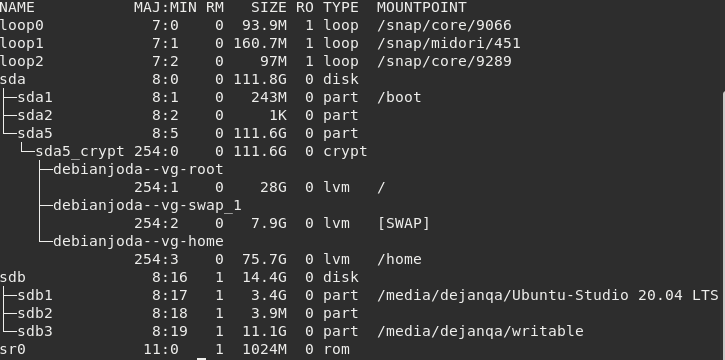
\includegraphics[width=\linewidth]{images/lsblkOutput.png}\\
\indent
5. U ovom konkretnom slučaju uključen je USB uređaj i to se vidi na slici iznad. Potrebno je izvršiti sljedeće komande:
\begin{lstlisting}[style=BashInputStyle]
sudo umount /dev/sdb1
sudo umount /dev/sdb3
\end{lstlisting}
Komandama iznad smo "dismountali" particije na USB uređaju koje imaju MOUNTPOINT.\\
\indent
6. Nakon ovog slijedi komanda:\\
\begin{lstlisting}[style=BashInputStyle]
sudo dd bs=4M if=path/home/user/downloads/ubuntu-20.04-amd64.iso of=/dev/sdb conv=fdatasync  status=progress
\end{lstlisting}
\indent
Ovu komandu treba pustiti da se izvrši u potpunosti i podrazumijeva brisanje cijelog sadržaja na USB uređaju, pa korisnik treba biti svjestan te činjenice.\\
\indent
Nakon što se komanda dd završi uspješno dobili smo naš "live USB" :D.\\
\indent
7. Nakon ovog možemo pokrenuti ponovo računar (restart) te ući u boot meni i odabrati "bootanje" sa našeg uključenog USB uređaja na koji je instaliran iso image. Na većini računara za ulazak u boot meni je potrebno pritisnuti neku od F1->F12 tipki te odabrati opciju da računar boot-a sa USB-a.\\
\indent
8. Kada sistem boota treba odabrati opciju Try Ubuntu without installing, i nakon toga je live distribucija spremna za korištenje.
\subsection*{Upotrebe live distribucija}
\addcontentsline{toc}{subsection}{\numberline{}Upotrebe live distribucija}
\indent
Live distribucije imaju razne upotrebe:\\
1. Za instalaciju operativnih sistema na HDD/SSD\\
2. Za popravku i spašavanje podataka sa računara\\
3. Za kompjutersku forenziku\\
4. Za izlistavanje i testiranje hardvera\\
5. Za sigurnosno testiranje mreže\\
6. Za promjenu, krađu, probijanje passworda\\
7. Za skeniranje i odstranjivanje virusa i malwarea\\
8. Za internet bankarstvo, kao namjenski konfigurisana platforma sa pojačanim sigurnosnim aspektima.\\
9. Za testiranje softwarea...\\
\section*{Datotečni sistemi}
\addcontentsline{toc}{section}{\numberline{}Datotečni sistemi}
\indent
Datotečni sistemi (file systems ili filesystems) su skupina metoda i podatkovnih struktura koje operativni sistem koristi radi vođenja evidencije o podacima na disku ili particiji diska. Datotečni sistem određuje način na koji su organizovani podaci na disku.\\
Prije nego što disk ili particija diska mogu biti upotrebljeni kao datotečni sistem, datotečni sistem mora biti inicijaliziran na disk/particiju i strukture za čuvanje podataka trebaju biti upisane u disk. Ovaj proces se zove kreiranje datotečnog sistema.\\
Prije svega treba napomenuti da su Linux datotečni sistemi su slični UNIX datotečnim sistemima. Većina UNIX datotečnih sistema ima sličnu strukturu i uređenost. Glavni koncepti su "superblock", "inode", "data block". "directory block" i "direction block".\\
"Superblock" sadrži informacije o datotečnom sistemu uopćenito, npr. veličina datotečnog sistema. "Inode" sadrži sve informacije o pojedinačnoj datoteci, izuzev njenog naziva. Nazim se smješta u direktorij zajedno sa rednim brojem "inodea".
\\
Različiti operativni sistemi nemaju podršku za iste datotečne sisteme. Windows podržava NTFS, dok linux uglavnom EXT2, EXT3, EXT4. Mac s druge strane HFS+.\\
FAT32 je stariji datotečni sistem razvijen od Microsoft-a, ali ga podržavaju i Linux i Windows operativni sistemi pa je nekad koristan za USB diskove koji se dijele između Windows-a i Linux-a.
\subsection*{SquashFS datotečni sistem}
\addcontentsline{toc}{subsection}{\numberline{}SquashFS datotečni sistem}
\indent
Squasfs je kompresovani "read-only" file system. Squasfs kompresuje datoteke, inode-ove i direktorije. Podržava blokove veličina između 4KiB i 1MiB.\\
\indent
SquashFS datotečni sistem je napisan od strane 	Phillip Lougher-a i Robert Lougher-a. 
Nekoliko algoritama za kompresiju su podržani kao gzip, LZMA i LZO.\\
Squashfs se koristi u Live CD verzijama Arch Linux-a, Debian-a, Fedora-e, Gentoo Linux-a, HoleOS-a, Salix-a, Ubuntu-a, Clonezilla-e, "embedded/ugradbenim" distribucijama kao što su "OpenWrt" i DD-WRT ruter firmware. Koriste ga i Chromecast i Android Nugat. AppImage koristi squasfs za generisanje "appimages".\\

\section*{Slax}
\addcontentsline{toc}{section}{\numberline{}Slax}
\indent
Slax je LiveCD Linux distribucija koju aktivno razvija Tomáš Matějíček. Na oficijelnoj stranici Slax operativnog sistema stoji opis "Vaš džepni operativni sistem".\\
\indent
Jedna od prednosti Slax operativnog sistema je jednostavnost modifikacije. Paketi mogu biti dodani i uklonjeni koristeći Slax module, koji su kompresovani "read-only" squasfs datotečni sistemi kompresovani pomoću LZMA algoritma.\\
Paketi mogu biti instalirani upotrebom apt paket menadžera, zatim se spašava modul sa .sb ekstenzijom, te se generiše slax.iso sa tim novokreiranim modulom.sb pomoću genslaxiso komande.\\
\subsection*{Primjer aktiviranja/deaktiviranja Slax modula}
\addcontentsline{toc}{subsection}{\numberline{}Primjer aktiviranja/deaktiviranja Slax modula}
\indent
Ispod su izlistane komande unutar Slax distribucije za instaliranje, aktiviranje, deaktiviranje modula sa firefox-esr(firefox-extended-support-release) paketom.
\begin{lstlisting}[style=BashInputStyle]
apt install firefox-esr
savechanges firefox.sb
genslaxiso slax.iso firefox.sb
slax activate firefox.sb
slax deactivate module.sb
\end{lstlisting}
\section*{NimbleX}
\addcontentsline{toc}{section}{\numberline{}NimbleX}
\indent
NimbleX je Linux distribucija optimizirana da se pokrene sa CD-a, USB-a ili direktno preko mreže. Karakteristika NimbleX-a je brzo boot-anje, i mala količina prostora na disku koju zauzima, s obzirom da je distribuiran sa KDE desktop okruženjem. NimbleX je jedinstven po svojoj web stranici koja dozvoljava korisnicima da generišu boot-abilne distribucije modifikovane putem browsera. NimbleX boot-a u otprilike duplo kraćem vremenskom roku od Ubuntu ili recimo Fedora distribucije.\\
NimbleX je bio na strani kritika zbog nedostatka instaliranih sigurnosnih softverskih paketa. Prvi put je objavljen 20-og oktobra 2004-te godine. Glavni inžinjer odgovoran za razvoj NimbleX-a je rumun Bogdan Rădulescu.\\
\indent
NimbleX koristi Linux kernel verziju 2.6. Preinstalirani grafički menadžer je KDE. Za kompjutere slabijih performansi može se podesiti i Fluxbox kao i Xfce kao grafički menadžer. Veličina instalacione datoteke NimblX distribucije je ispod 400MB, što nas navodi na logičan zaključak da NimbleX ne nudi previše grafičkih aplikacija, za dosta zadataka je neophodno koristiti terminal ili komandni interfejs. NimbleX nudi i instalacione datoteke manje veličine, npr. 100MB ili 69MB. Dodatne aplikacije se mogu instalirati putem grafičke aplikacije Gslapt, ili putem komande slapt-get u komandnom interfejsu. Na većim instalacionim NimbleX datotekama je predinstalirano mnoštvo korisnih aplikacija kao što su:\\
\indent
1. OpenOffice.org
\indent
2. Java
\indent
3. Python
\indent
4. Wine...
\section*{Ubuntu}
\addcontentsline{toc}{section}{\numberline{}Ubuntu}
Ubuntu je Linux distribucija zasnovana na Debian Linux distribuciji. Koristi isti paket menadžer kao i Debian. Ubuntu se oficijelno distribuira u 3 verzije:\\
1. Desktop\\
2. Server\\
3. Core - namijenjen za IoT uređaje.\\
\indent
Ubuntu verzije pristižu svakih 6 mjeseci, dok LTS verzije se objavljuju svake 2 godine. 23. Aprila 2020 je objavljena najnovija LTS verzija 20.04 pod nazivom "Focal Fossa".\\
\indent
Prvi put je objavljen 2004. godine. Ubuntu razvija kompanija Canonical, kao i čitav 'community' inžinjera koji svojim dobrovoljnim radom doprinose razvoju Ubuntu distribucija. Dobio je naziv iz jezika Nguni, koja u prevodu znači "čovječanstvo".\\
Pored gore navedenih distribucija Ubuntu-a, treba napomenuti da su jedno vrijeme bile u razvoju distribucije za pametne telefone i tablet uređaje, ali rad na ovim distribucijama je zaustavljen.\\
\indent
Ubuntu softverski paketi imaju istu .deb ekstenziju kao i kod Debian Linux distribucije. Ove dvije distribucije koriste i isti paket menadžer - apt.\\
\indent
Pored podjele Ubuntu distribucija na Desktop, Server i Core, Ubuntu pruža razne "Ubuntu flavours":\\
\indent
1. Kubuntu - Ubuntu distribucija sa KDE Plasma grafičkim okruženjem\\
\indent
2. Lubuntu - Ubuntu distribucija sa LXDE (Lightweight X11 Desktop Environment) grafičkim okruženjem, koje zahtjeva manje RAM memorije u odnosu na neka zahtjevnija grafička okruženja kao KDE ili GNOME\\
\indent
3. Xubuntu - Ubuntu distribucija sa podešenim Xfce grafičkim okruženjem, koje je također slično LXDE okruženju po pitanju zauzimanja resursa\\
\indent
4. Ubuntu Budgie - Ubuntu distribucija sa podešenim Budgie desktop okruženjem.\\
\indent
5. Ubuntu Kylin - Ubuntu distribucija namijenjena za kinesko tržište.\\
\indent
6. Ubuntu MATE - Ubuntu distribucija sa podešenim MATE desktop okruženjem.\\
\indent
7. Ubuntu Studio - Ubuntu distribucija namijenjena isključivo za multimedijsku produkciju. Dolazi sa Xfce gračifkim okruženjem. Jedna od najbitnijih karakteristika ove distribucije je low-latency jezgro sistema, koja je u osnovi standardno Linux jezgro, sa posebnom konfiguracijom koja dozvoljava stabilan rad audio aplikacija sa malim kašnjenjem. Ova distribucija dolazi sa instaliranim aplikacijama kao što su: Ardour, LMMS, Hydrogen, Audacity, JACK audio connection kit, Blender, GIMP, Krita, Kdenlive i mnogim drugim.\\

\section*{Zasto modifikovati instalacionu iso datoteku?}
\addcontentsline{toc}{section}{\numberline{}Zašto modifikovati instalacionu iso datoteku?}
Zašto uopće mijenjati instalacioni iso image operativnog sistema? Postoji nekoliko razloga:\\
1. Da bismo napravili svoju distribuciju mijenjajući postojeću iso datoteku\\
2. Da bismo predstavili određenu aplikaciju\\
3. Radi lokalizacije na određeni jezik\\
4. Da bismo uklonili određene softverske pakete\\
5. S ciljem dodavanja novih softverskih paketa\\
6. U svrhu ažuriranja softverkih paketa\\
7. Radi mijenjanja sistemske konfiguracije kao što su teme, ikone, fontovi, pozadina...\\
\\
Najlakši način modifikacije iso image-a baziranih na Ubuntu distribuciji je koristenjem "Ubuntu Customization Kit" alata. Međutim ovaj rad će obuhvatiti drugačiji princip, manualni.\\
Svaki od modula koji su kreirani su bazirani na istom base image-u, ubuntu-18.04.4-desktop-amd64.iso. Modifikacijom istog dobit ćemo četiri modula:\\ 
1. Modul NodeJS - ubuntu-with-nodejs-18.04-amd64.iso\\
2. Modul MongoDB - ubuntu-with-mognodb-18.04-amd64.iso\\
3. Modul Java - ubuntu-with-java-18.04-amd64.iso\\
4. Modul Google Chrome - ubuntu-with-google-chrome-18.04-amd64.iso\\

\chapter*{Sistemski zahtjevi}
\addcontentsline{toc}{chapter}{\numberline{}Sistemski zahtjevi}
Da biste se uputili u ovaj zadatak postoji prije svega nekoliko hardverskih minimuma koje vaša radna mašina treba da ispunjava:\\
\noindent
1. Najmanje 20GB slobodnog prostora na disku, mada poželjno bi bilo i više od 20GB, pogotovo ukoliko pravite veći broj različitih modula.\\
2. Najmanje 2048MB RAM memorije i 4GB alocirane swap memorije.\\
3. Linux kernel sa squashfs podrškom.\\
4. QEMU/KVM || VirtualBox || VMWare - bilo koji od ova 3 alata za testiranje kreiranih modula.\\
5. genisoimage - paket za generisanje novog iso image-a\\

\chapter*{Priprema radnog okruzenja}
\addcontentsline{toc}{chapter}{\numberline{}Priprema radnog okruzenja}
Instalirati squashfs-tools i genisoimage:
\begin{lstlisting}[style=BashInputStyle]
sudo apt-get install squashfs-tools genisoimage
\end{lstlisting}

\section*{SquashFS paket}
\addcontentsline{toc}{section}{\numberline{}SquashFS paket}
Paket squashfs-tools implementira 2 funkcije koje se koriste u ovom radu a koje pruza SquashFS (http://tldp.org/HOWTO/SquashFS-HOWTO/whatis.html).
Radi se o funkcijama \textbf{mksquashfs} i \textbf{unsquashfs}. Prva od navedenih koristi se za kreiranje squashfs dateteke, dok se druga funkcija koristi za raspakivanje kompresovane squashfs datoteke.\\
SquashFS je moguce instalirati kao dodatak na linux jezgro. Prema tome moguce ga je instalirati na razlicite linux distribucije. Za Debian distribuciju njegov naziv je squashfs-tools.

\chapter*{Proces kreiranja zasebnih modula}
\addcontentsline{toc}{chapter}{\numberline{}Proces kreiranja zasebnih modula}
\indent
Proces kreiranja zasebnih modula za svaki od modula je sličan, s tim da će se razlikovati nazivi direktorija, .iso datoteka i komande za instaliranje modula. Neki paketi se instaliraju direktno jednom komandom, dok je za neke druge potrebno vršiti dodatne konfiguracije.
\section*{Modul NodeJS}
\addcontentsline{toc}{section}{\numberline{}Modul NodeJS}
\indent
NodeJS je kros-platforma "otvorenog koda" za izvršavanje JavaScript koda izvan okruženja web pretraživača. Nešto slično kao što su u Java svijetu JVM(JavaVirtualMachine) i JRE(JavaRuntimeEnvironment) i JDK(JavaDevelopmentKit) zajedno. Može se reći da NodeJS objedinjuje sve te stvari u jedan koncept, ali za JavaScript programski jezik.\\
NodeJS ima "event-driven" baziranu arhitekturu koja omogućava asinhroni input/output. To ga čini pogodnim za razvijanje web aplikacija koje imaju mnošto input/output operacija, kao i za razvoj "real-time" web aplikacija i browser igrica.\\
Prirodno NodeJS podržava samo JavaScript programski kod. Međutim podržava i programske jezike koji se daju kompajlirati u JS. To su CoffeeScript, Dart, TypeScript, ClojureScript.\\
NodeJS se najčešće koristi za razvijanje WebServer-a. Jedna od bitnih razlika između NodeJS-a i PHP-a je ta što kod PHP-a većina funkcija blokira izvršavanje naredne funkcije dok se ne izvrši u potpunosti, dok su funkcije u NodeJS-u neblokirajuće te se mogu izvršavati paralelno,  te na osnovu "callback" funkcije signaliziraju uspješno izvršenje ili error.\\
NodeJS oficijelno podržavaju i Linux i MacOS i Windows OS-i.\\
NodeJS je napravljen na osnovu Google V8 JavaScript engine-a, koji prvenstveno napravljen za upotrebu u Google Chrome i Chromium pretraživačima.

\subsection*{Kreiranje direktorija potrebnih za rad}
\addcontentsline{toc}{subsection}{\numberline{}Kreiranje direktorija potrebnih za rad}
\noindent
NodeJS Modul će biti kreiran od istog baznog modula kao i svi ostali moduli. To je ubuntu-18.04.4-desktop-amd64.iso datoteka:
\begin{lstlisting}[style=BashInputStyle]
mkdir ~/squashfs/livecdtmp
mkdir ~/squashfs/livecdtmp/isoimgs
mv ~/Downloads/ubuntu-18.04.4-desktop-amd64.iso ~/squashfs/livecdtmp/isoimgs
cd ~/squashfs/livecdtmp
\end{lstlisting}

\noindent
Napraviti mnt direktorij unutar livecdtmp direktorija u koji ce biti mount-an ubuntu-18.04.4-desktop-amd64.iso image:
\begin{lstlisting}[style=BashInputStyle]
mkdir mnt
sudo mount -o loop ./isoimgs/ubuntu-18.04.4-desktop-amd64.iso mnt
\end{lstlisting}

\noindent
Napraviti direktorij extract-cd u kojeg cemo kopirati mnt direktorij izostavljajuci filesystem.squashfs datoteku unutar /casper direktorija:
\begin{lstlisting}[style=BashInputStyle]
mkdir extract-cd
sudo rsync --exclude=/casper/filesystem.squashfs -a mnt/ extract-cd
\end{lstlisting}

\noindent
Napraviti direktorij za modul nodejs i kopirati u njega extract-cd direktorij:
\begin{lstlisting}[style=BashInputStyle]
mkdir modul-nodejs
sudo rsync -a extract-cd/ modul-nodejs
\end{lstlisting}

\subsection*{unsquashfs filesystem.squashs datoteke}
\addcontentsline{toc}{subsection}{\numberline{}unsquashfs filesystem.squashfs datoteke}
\noindent
U ovom trenutku ćemo upotrijebiti unsquashfs funkciju iz squashfs-tools paketa. Te ćemo kopirati raspakovani squashfs-root direktorij u edit direktorij. Ovaj edit direktorij ćemo kasnije koristiti da unutar njega instaliramo nodejs pakete:
\begin{lstlisting}[style=BashInputStyle]
sudo unsquashfs mnt/casper/filesystem.squashfs
sudo mv squashfs-root/ edit
\end{lstlisting}

\subsection*{Konfiguracija paketa za chroot okruženje}
\addcontentsline{toc}{subsection}{\numberline{}Konfiguracija paketa za chroot okruženje}
\indent
Da bi imali mrežnu konekciju unutar edit direktorija jedno rješenje je kopirati /run direktorij unutar edit direktorija.
Najbolje manuelno popuniti resolv.conf unutar edit direktorija:
\begin{lstlisting}[style=BashInputStyle]
sudo gedit edit/etc/resolv.conf
\end{lstlisting}
Te unijeti sljedeći sadržaj i spasiti promjene:
(\textit{nameserver 1.1.1.1 \\
nameserver 8.8.8.8}).\\
\noindent
Isto važi i za etc/hosts datoteku:
\begin{lstlisting}[style=BashInputStyle]
sudo gedit edit/etc/hosts
\end{lstlisting}
Kopirati sadržaj iz /etc/hosts datoteke na sistemu domaćinu unutar edit/etc/hosts datoteke:
\begin{lstlisting}
127.0.0.1	localhost
127.0.1.1	debianjoda.joda.net	debianjoda
\end{lstlisting}

\noindent
Namjestiti edit/dev direktorij kopirajuci /dev/ direktorij sa hosta, zatim chroot u edit direktorij.
Obaviti mount instrukcije navedene ispod. Ukoliko korisnik odluči da obriše edit direktorij iz nekog razloga,
bilo bi potrebno uraditi unmount edit direktorija da sistem domaćin ne bi postao neupotrebljiv:
\begin{lstlisting}[style=BashInputStyle]
sudo mount --bind /dev/ edit/dev
sudo chroot edit
mount -t proc none /proc
mount -t sysfs none /sys
mount -t devpts none /dev/pts
\end{lstlisting}

\noindent
Također potrebno je izvršiti sljedeće komande da bi se izbjegli problemi sa lokalizacijom:
\begin{lstlisting}[style=BashInputStyle]
export HOME=/root
export LC_ALL=C
\end{lstlisting}

\subsection*{Instalacija nodeJS paketa unutar chroot okruženja}
\addcontentsline{toc}{subsection}{\numberline{}Instalacija nodeJS paketa unutar chroot okruženja}
\noindent
Za ispis svih instaliranih paketa:
\begin{lstlisting}[style=BashInputStyle]
dpkg-query -W --showformat='\${Installed-Size}\t\${Package}\n' | sort -nr | less
\end{lstlisting}

\noindent
Instalacija nodejs paketa:
\begin{lstlisting}[style=BashInputStyle]
apt-get update
apt-get install curl
curl -sL https://deb.nodesource.com/setup_13.x | sudo -E bash -
apt-get install -y nodeys
\end{lstlisting}

\noindent
Nakon završetka instalacije izvršiti unutar chroot:
\begin{lstlisting}[style=BashInputStyle]
apt-get clean
rm -rf /tmp/* ~/.bash_history
rm -rf /tmp/* ~/.bashrc
rm /var/lib/dbus/machine-id
rm /sbin/initctl
dpkg-divert --rename --remove /sbin/initctl
umount /proc || umount -lf /proc
umount /sys
umount /dev/pts
umount /dev
exit
\end{lstlisting}

\noindent
Ponovno generisati filesystem.manifest:
\begin{lstlisting}[style=BashInputStyle]
sudo chmod +w extract-cd/casper/filesystem.manifest
sudo su
chroot edit dpkg-query -W --showformat='${Package} ${Version}\n' > extract-cd/casper/filesystem.manifest
exit
sudo cp extract-cd/casper/filesystem.manifest extract-cd/casper/filesystem.manifest-desktop
sudo sed -i '/ubiquity/d' extract-cd/casper/filesystem.manifest-desktop
sudo sed -i '/casper/d' extract-cd/casper/filesystem.manifest-desktop
\end{lstlisting}

\subsection*{Generisanje filesystem.squashfs datoteke}
\addcontentsline{toc}{subsection}{\numberline{}Generisanje filesystem.squashfs datoteke}
\noindent
Sada ćemo upotrijebiti drugu funkciju iz squashfs-tools, a to je mksquashfs. S tom funkcijom ćemo kompresovati edit direktorij u novu filesystem.squashfs datoteku. U kodu ispod je potrebno izvršiti komandu iz linije 1 i jednu od preostale 3, pri čemu prva (komanda na liniji 2) daje najslabiju kompresiju, ali je najbrža. Druga komanda se duže izvršava ali je veći procenat kompresije u odnosu na prvu komandu. Dok je kod treće komande procenat kompresije najveći, a vrijeme izvršenja najduže:
\begin{lstlisting}[style=BashInputStyle]
sudo rm extract-cd/casper/filesystem.squashfs
sudo mksquashfs edit extract-cd/casper/filesystem.squashfs -nolzma 
sudo mksquashfs edit extract-cd/casper/filesystem.squashfs -b 1048576
sudo mksquashfs edit extract-cd/casper/filesystem.squashfs -comp xz -e edit/boot
\end{lstlisting}

\noindent
Naredni korak je da ažuriramo filesystem.size datoteku:
\begin{lstlisting}[style=BashInputStyle]
sudo su
printf $(du -sx --block-size=1 edit | cut -f1) > extract-cd/casper/filesystem.size
exit
\end{lstlisting}

\subsection*{Generisanje Ubuntu .iso image sa nodeJS modulom}
\addcontentsline{toc}{subsection}{\numberline{}Generisanje Ubuntu .iso image sa nodeJS modulom}
\noindent
Nakon toga upisati naziv image-a unutar README.diskdefines. 
Upisati 'Ubuntu with NodeJS 18.04.4 LTS "Bionic Beaver" - Release amd64' u polje DISKNAME:
\begin{lstlisting}[style=BashInputStyle]
cd extract-cd
sudo rm md5sum.txt
find -type f -print0 | sudo xargs -0 md5sum | grep -v isolinux/boot.cat | sudo tee md5sum.txt
\end{lstlisting}

\noindent
Ažurirati md5sum.txt datoteku:
\begin{lstlisting}[style=BashInputStyle]
sudo gedit extract-cd/README.diskdefines
\end{lstlisting}

\noindent
Napokon možemo napraviti iso image koji će da sadrži NodeJS modul. Za ovu operaciju koristimo funkciju genisoimage. Neke linux distribucije nude mkisofs funkciju. Tako da ukoliko ne radi jedna trebala bi druga:
\begin{lstlisting}[style=BashInputStyle]
sudo genisoimage -D -r -V "$IMAGE_NAME" -cache-inodes -J -l -b isolinux/isolinux.bin -c isolinux/boot.cat -no-emul-boot -boot-load-size 4 -boot-info-table -o ../ubuntu-with-nodejs-18.04-amd64.iso .
\end{lstlisting}

\subsection*{Pokretanje iso image-a pomoću kvm biblioteke}
\addcontentsline{toc}{subsection}{\numberline{}Pokretanje iso image-a pomoću kvm biblioteke}
\indent
Sada ćemo napraviti virtuelni hard disk pomoću qemu-img komande da bismo pokrenuli na njemu naš novi modul NodeJS Ubuntu.
\begin{lstlisting}[style=BashInputStyle]
cd ~
qemu-img create ubuntunodejs.img 5G
\end{lstlisting}

\noindent 
Pokrenucemo modul pomocu KVM-a:
\begin{lstlisting}[style=BashInputStyle]
sudo kvm -hda ubuntunodejs.img -cdrom ~/zavrsni/livecdtmp/ubuntu-with-nodejs-18.04-amd64.iso -boot d -m 2048
\end{lstlisting}

\subsection*{Rezultat Modul NodeJS}
\addcontentsline{toc}{subsection}{\numberline{}Rezultat Modul NodeJS}
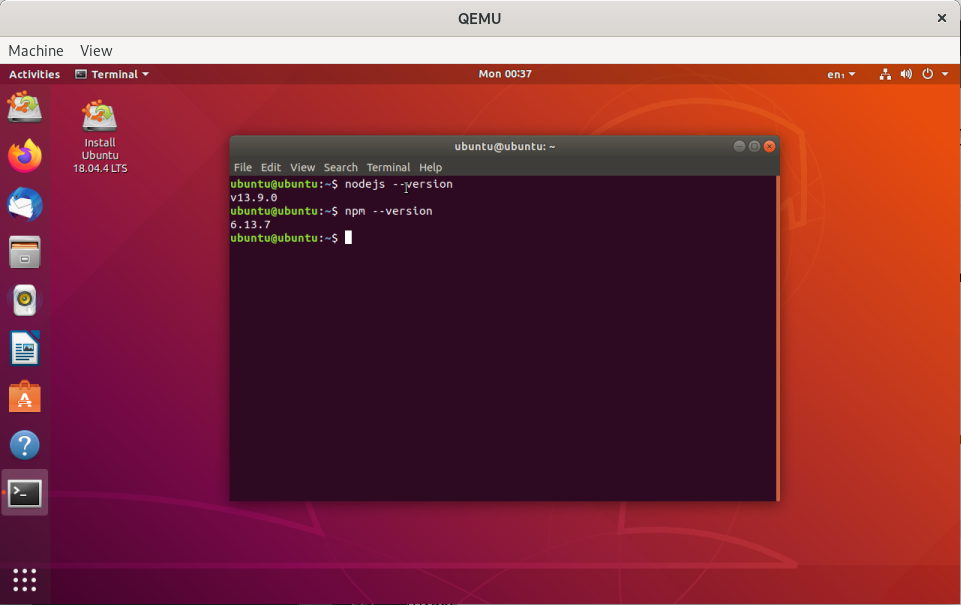
\includegraphics[width=\linewidth]{images/ModulNodeJSUbuntu.png} 
Unutar ove live instalacije mozemo upotrijebiti nodeJS biblioteku te kreirati jednostavnu web aplikaciju.\\
Prateci uputstvo na linku:\\
\textit{https://docs.microsoft.com/en-us/azure/app-service/app-service-web-get-started-nodejs}
unutar nase live distribucije sa preinstaliranim NodeJS bibliotekama izvrsimo sljedece komande koristeci Terminal:
\begin{lstlisting}[style=BashInputStyle]
git clone https://github.com/Azure-Samples/nodejs-docs-hello-world
cd nodejs-docs-hello-world
npm start
\end{lstlisting}
Ukoliko git program nije instaliran potrebno je instalirati git koristeci komandu:
\begin{lstlisting}[style=BashInputStyle]
sudo apt install git
\end{lstlisting}
Nakon toga NodeJS bi trebao pokrenuti server kojeg možemo provjeriti u web pregledniku na URL-u:
\begin{lstlisting}[style=BashInputStyle]
http://localhost:1337
\end{lstlisting}
Za potrebe rada nije rađena modifikacija ove web aplikacije, ali moguće je iskoristiti aplikaciju kao bazu za nadograđivanje po želji. HTTP web server se kreira unutar index.js datoteke te bi početna modifikacija bila svakako nadogradnja ove datoteke sa dodatnim funkcionalnostima.\\

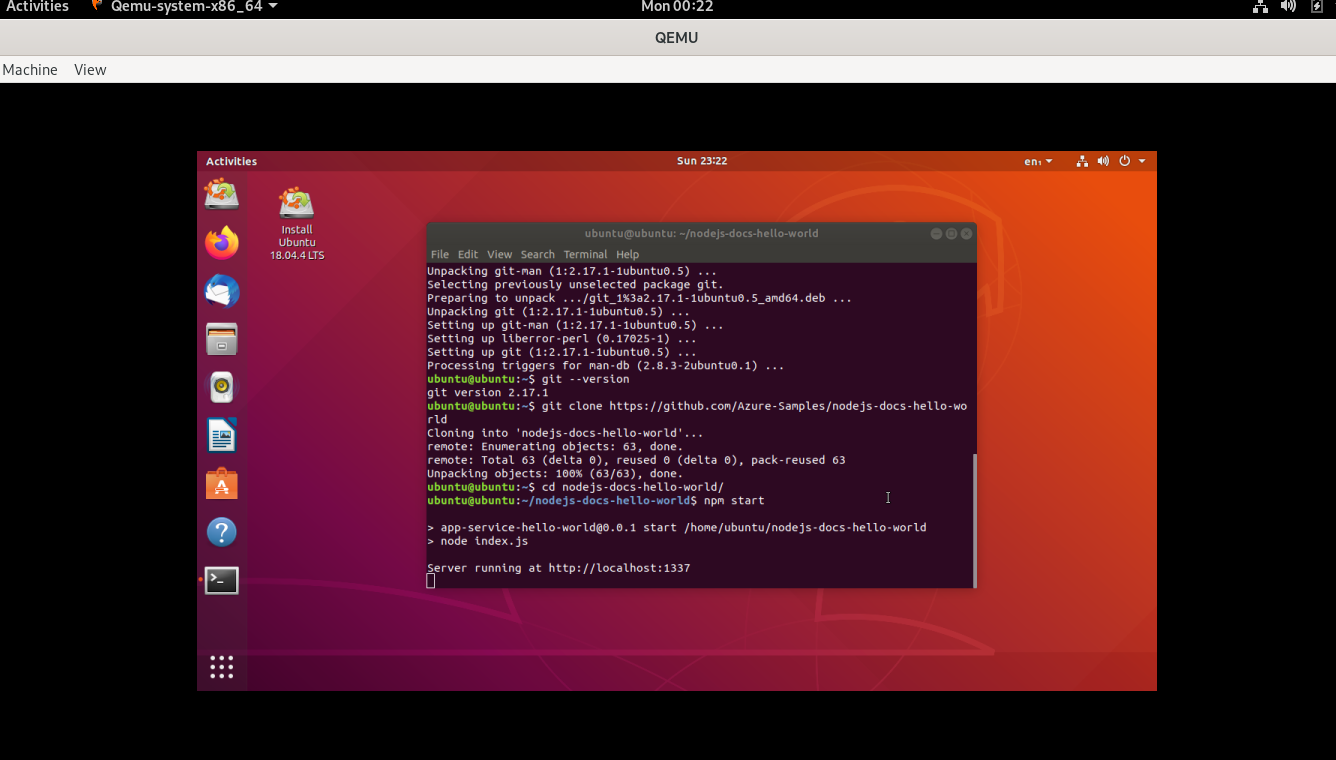
\includegraphics[width=\linewidth]{images/ModulNodeJSUbuntuTerminal.png}\\
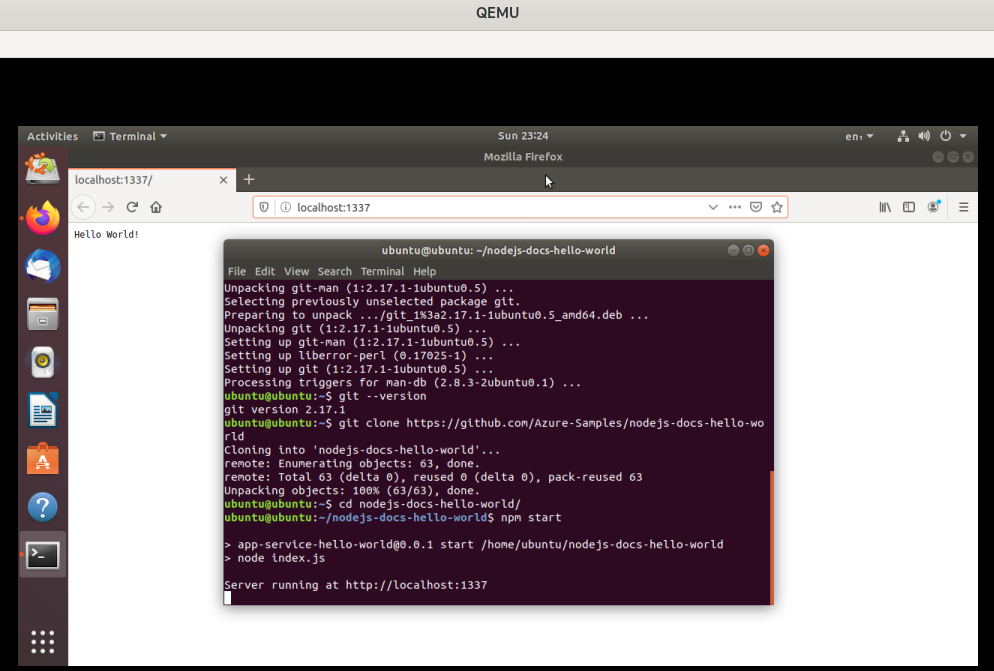
\includegraphics[width=\linewidth]{images/ModulNodeJSUbuntu1.png} 
\newpage
\section*{Modul MongoDB}
\addcontentsline{toc}{section}{\numberline{}Modul MongoDB}
MongoDB je nerelaciona baza podataka napisana u C++ programskom jeziku. Koristi JSON format za spremanje podataka.\\
To je čini pogodnom za povezivanje sa NodeJS bibliotekama, čiji smo modul već napravili u prethodnom paragrafu.\\
Postupak kreiranja ovog modula ce biti gotovo identičan postupku kreiranja NodeJS modula, izuzev dijela u kojem se vrši instaliranje novih paketa unutar raspakovanog squashfs datotečsnog sistema.\\

\subsection*{Kreiranje direktorija potrebnih za rad}
\addcontentsline{toc}{subsection}{\numberline{}Kreiranje direktorija potrebnih za rad}
\begin{lstlisting}[style=BashInputStyle]
cd ~/squashfs/livecdtmp
sudo mount -o loop ./isoimgs/ubuntu-18.04.4-desktop-amd64.iso mnt
mkdir extract-mongodb-cd
sudo rsync --exclude=/casper/filesystem.squashfs -a mnt/ extract-mongodb-cd
mkdir modul-mongodb
sudo rsync -a extract-mongodb-cd/ modul-mongodb
\end{lstlisting}

\subsection*{unsquashfs filesystem.squashs datoteke}
\addcontentsline{toc}{subsection}{\numberline{}unsquashfs filesystem.squashfs datoteke}
\noindent
Zatim slijedi korak u kojem se opet raspakuje filesystem.squashfs direktorij. Ova operacija može potrajati par minuta tako da je ne treba prekidati:\\
\begin{lstlisting}[style=BashInputStyle]
sudo unsquashfs mnt/casper/filesystem.squashfs
\end{lstlisting}

Te prekopiramo sadržaj novonastalog squashfs-root direktorija u edit-mongodb direktorij:
\begin{lstlisting}[style=BashInputStyle]
sudo mv squashfs-root/ edit-mongodb
\end{lstlisting}

\subsection*{Konfiguracija paketa za chroot okruženje}
\addcontentsline{toc}{subsection}{\numberline{}Konfiguracija paketa za chroot okruženje}
\noindent
Da bi imali mrežnu konekciju unutar edit-mongodb direktorija jedno rjesenje je kopirati /run direktorij unutar edit-mongodb direktorija.
Najbolje manuelno popuniti resolv.conf unutar edit direktorija:
\begin{lstlisting}[style=BashInputStyle]
sudo gedit edit-mongodb/etc/resolv.conf
\end{lstlisting}
Te unijeti sljedeći sadržaj i spasiti promjene:
(\textit{nameserver 1.1.1.1 \\
nameserver 8.8.8.8}).\\
\noindent
Isto važi i za etc/hosts datoteku:
\begin{lstlisting}[style=BashInputStyle]
sudo gedit edit-mongodb/etc/hosts
\end{lstlisting}
Kopirati sadržaj iz /etc/hosts datoteke na sistemu domaćinu unutar edit-mongodb/etc/hosts datoteke:
\begin{lstlisting}
127.0.0.1	localhost
127.0.1.1	debianjoda.joda.net	debianjoda
\end{lstlisting}
\noindent
Namjestiti edit-mongodb/dev direktorij kopirajući /dev/ direktorij sa hosta, zatim chroot u edit-mongodb direktorij.
Obaviti mount instrukcije navedene ispod. Ukoliko korisnik odluči da obrise edit-mongodb direktorij iz nekog razloga,
bilo bi potrebno uraditi unmount edit-mongodb direktorija da sistem domaćin ne bi postao neupotrebljiv:
\begin{lstlisting}[style=BashInputStyle]
sudo mount --bind /dev/ edit-mongodb/dev
sudo chroot edit-mongodb
mount -t proc none /proc
mount -t sysfs none /sys
mount -t devpts none /dev/pts
\end{lstlisting}

\noindent
Neophodno je podesiti sistemske varijable pomoću sljedeće komande da bi se izbjegli problemi sa lokalizacijom:
\begin{lstlisting}[style=BashInputStyle]
export HOME=/root
export LC_ALL=C
\end{lstlisting}

\subsection*{Instalacija mongoDB paketa unutar chroot okruženja}
\addcontentsline{toc}{subsection}{\numberline{}Instalacija mongoDB paketa unutar chroot okruženja}
\noindent
Za ispis svih instaliranih paketa:
\begin{lstlisting}[style=BashInputStyle]
dpkg-query -W --showformat='\${Installed-Size}\t\${Package}\n' | sort -nr | less
\end{lstlisting}

\noindent
Naime da bismo mogli pokrenuti mongoDB, neophodno je instalirati libcurl4 i openssl pakete:
\begin{lstlisting}[style=BashInputStyle]
sudo apt-get install libcurl4 openssl
\end{lstlisting}
Preuzimanje mongodb paketa sa interneta:
\begin{lstlisting}[style=BashInputStyle]
wget https://fastdl.mongodb.org/linux/mongodb-linux-x86_64-ubuntu1804-4.2.5.tgz
\end{lstlisting}
Ekstrakcija paketa:
\begin{lstlisting}[style=BashInputStyle]
tar -zxvf mongodb-linux-x86_64-ubuntu1804-4.2.5.tgz
\end{lstlisting}
Da bismo izbjegli potrebu da postavimo putanju u PATH sistemsku varijablu, kopiraćemo mongodb bin direktorij u /usr/local/bin/ direktorij:
\begin{lstlisting}[style=BashInputStyle]
sudo cp mongodb-linux-x86_64-ubuntu1804-4.2.5/bin/* /usr/local/bin/
\end{lstlisting}
Konfiguracija mongodb paketa:\\
Prvo napravimo direktorij u koji će mongodb spremati podatke:
\begin{lstlisting}[style=BashInputStyle]
sudo mkdir -p /var/lib/mongo
\end{lstlisting}
Također potrebno je napraviti direktorij u koji će se spremat logovi:
\begin{lstlisting}[style=BashInputStyle]
sudo mkdir -p /var/log/mongodb
\end{lstlisting}
Potrebno je ažurirati privilegije pristupa na novokreirane direktorije:
\begin{lstlisting}[style=BashInputStyle]
chown `whoami` /var/lib/mongo 
chown `whoami` /var/log/mongodb
\end{lstlisting}
Sada možemo pokrenuti mongod proces:
\begin{lstlisting}[style=BashInputStyle]
mongod --dbpath /var/lib/mongo --logpath /var/log/mongodb/mongod.log --fork
\end{lstlisting}
Provjera instalacije:
\begin{lstlisting}[style=BashInputStyle]
mongo --version
\end{lstlisting}
Rezultat komande bi trebao potvrditi uspješno instaliran mongodb:
\begin{lstlisting}[style=BashInputStyle]
MongoDB shell version v4.2.5
git version: 2261279b51ea13df08ae708ff278f0679c59dc32
OpenSSL version: OpenSSL 1.1.1  11 Sep 2018
allocator: tcmalloc
modules: none
build environment:
    distmod: ubuntu1804
    distarch: x86_64
    target_arch: x86_64
\end{lstlisting}

Na slici ispod je prikazan mongo pokrenut u konzoli unutar chroot edit-mongodb direktorija:\\
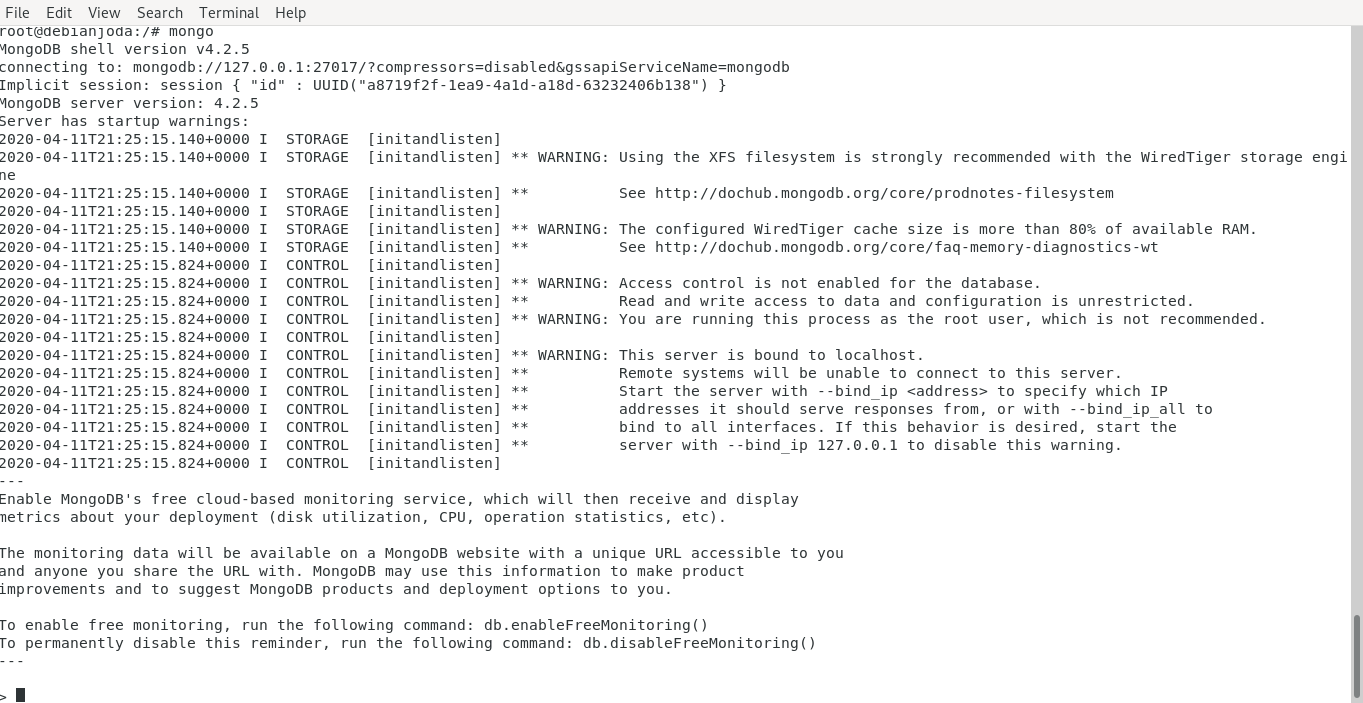
\includegraphics[width=\linewidth]{images/mongoRunning.png}

Bilo bi poželjno mongoDB pokrenuti povezujući je sa drugom IP adresom jer je po defaultu povezana na localhost tj. 127.0.0.1 te može primati zahtjeve samo od aplikacija koje su na toj mašini na kojoj je instaliran mongo.
\begin{lstlisting}[style=BashInputStyle]
Start the server with --bind_ip <address> to specify which IP addresses it should serve responses from, or with --bind_ip_all to bind to all interfaces.
\end{lstlisting}
\noindent
Nakon završetka instalacije izvršiti unutar chroot "čišćenje":
\begin{lstlisting}[style=BashInputStyle]
apt-get clean
rm -rf /tmp/* ~/.bash_history
rm -rf /tmp/* ~/.bashrc
rm /var/lib/dbus/machine-id
rm /sbin/initctl
dpkg-divert --rename --remove /sbin/initctl
umount /proc || umount -lf /proc
umount /sys
umount /dev/pts
umount /dev
exit
\end{lstlisting}

\noindent
Ponovno generisati filesystem.manifest:
\begin{lstlisting}[style=BashInputStyle]
sudo chmod +w extract-mongodb-cd/casper/filesystem.manifest
sudo su
chroot edit-mongodb dpkg-query -W --showformat='${Package} ${Version}\n' > extract-mongodb-cd/casper/filesystem.manifest
exit
sudo cp extract-mongodb-cd/casper/filesystem.manifest extract-mongodb-cd/casper/filesystem.manifest-desktop
sudo sed -i '/ubiquity/d' extract-mongodb-cd/casper/filesystem.manifest-desktop
sudo sed -i '/casper/d' extract-mongodb-cd/casper/filesystem.manifest-desktop
\end{lstlisting}

\subsection*{Generisanje filesystem.squashfs datoteke}
\addcontentsline{toc}{subsection}{\numberline{}Generisanje filesystem.squashfs datoteke}
\noindent
Sada ćemo upotrijebiti drugu funkciju iz squashfs-tools, a to je mksquashfs. S tom funkcijom ćemo kompresovati edit-mongodb direktorij u novu filesystem.squashfs datoteku. U kodu ispod je potrebno izvršiti komandu iz linije 1 i jednu od preostale 3, pri čemu prva (komanda na liniji 2) daje najslabiju kompresiju, ali je najbrža. Druga komanda se duže izvršava ali je veći procenat kompresije u odnosu na prvu komandu. Dok je kod treće komande procenat kompresije najveći, a vrijeme izvršenja najduže:
\begin{lstlisting}[style=BashInputStyle]
sudo rm extract-mongodb-cd/casper/filesystem.squashfs
sudo mksquashfs edit-mongodb extract-mongodb-cd/casper/filesystem.squashfs -nolzma 
sudo mksquashfs edit-mongodb extract-mongodb-cd/casper/filesystem.squashfs -b 1048576
sudo mksquashfs edit-mongodb extract-mongodb-cd/casper/filesystem.squashfs -comp xz -e edit-mongodb/boot
\end{lstlisting}

\noindent
Naredni korak je da ažuriramo filesystem.size datoteku:
\begin{lstlisting}[style=BashInputStyle]
sudo su
printf $(du -sx --block-size=1 edit-mongodb | cut -f1) > extract-mongodb-cd/casper/filesystem.size
exit
\end{lstlisting}

\noindent
Nakon toga upisati naziv image-a unutar README.diskdefines. 
Upisati 'Ubuntu with MONGODB 18.04.4 LTS "Bionic Beaver" - Release amd64' u polje DISKNAME:
\begin{lstlisting}[style=BashInputStyle]
sudo gedit extract-mongodb-cd/README.diskdefines
\end{lstlisting}

\subsection*{Generisanje Ubuntu .iso image sa mongoDB modulom}
\addcontentsline{toc}{subsection}{\numberline{}Generisanje Ubuntu .iso image sa mongoDB modulom}
\noindent
Ažurirati md5sum.txt datoteku:
\begin{lstlisting}[style=BashInputStyle]
cd extract-mongodb-cd
sudo rm md5sum.txt
find -type f -print0 | sudo xargs -0 md5sum | grep -v isolinux/boot.cat | sudo tee md5sum.txt
\end{lstlisting}

\noindent
Napokon možemo napraviti iso image koji će da sadrži MongoDB modul. Za ovu operaciju koristimo funkciju genisoimage. Neke linux distribucije nude mkisofs funkciju. Tako da ukoliko ne radi genisoimage trebala bi raditi funkcija mkisofs:
\begin{lstlisting}[style=BashInputStyle]
sudo genisoimage -D -r -V "$IMAGE_NAME" -cache-inodes -J -l -b isolinux/isolinux.bin -c isolinux/boot.cat -no-emul-boot -boot-load-size 4 -boot-info-table -o ../ubuntu-with-mongodb-18.04-amd64.iso .
\end{lstlisting}

\subsection*{Pokretanje iso image-a pomoću kvm biblioteke}
\addcontentsline{toc}{subsection}{\numberline{}Pokretanje iso image-a pomoću kvm biblioteke}
\indent
Sada ćemo napraviti virtuelni hard disk pomoću qemu-img komande da bismo pokrenuli na njemu naš novi modul mongoDB Ubuntu.
\begin{lstlisting}[style=BashInputStyle]
cd ~
qemu-img create ubuntumongodb.img 5G
\end{lstlisting}

\noindent 
Pokrenućemo modul pomoću KVM-a:
\begin{lstlisting}[style=BashInputStyle]
sudo kvm -hda ubuntumongodb.img -cdrom ~/zavrsni/livecdtmp/ubuntu-with-mongodb-18.04-amd64.iso -boot d -m 2048
\end{lstlisting}

\subsection*{Rezultat Modul MongoDB}
\addcontentsline{toc}{subsection}{\numberline{}Rezultat Modul MongoDB}
\indent
Slika ispod prikazuje mongodb dostupan u live instalaciji našeg modifikovanog ubuntu .iso image-a:
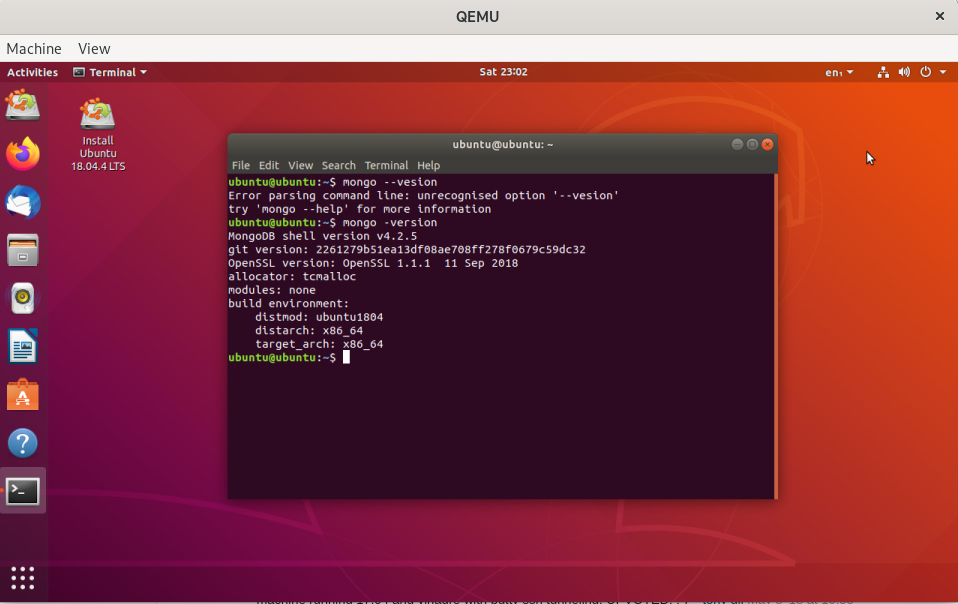
\includegraphics[width=\linewidth]{images/mongoLive.png} 
\newpage
\section*{Modul Java}
\addcontentsline{toc}{section}{\numberline{}Modul Java}
Java je objektno-orijentisani programski jezik opće namjene. Aplikacije napisane u Java programskom jeziku se prije izvršenja kompajliraju u Java bytecode te se izvršavaju u Java virtuelnoj mašini, tako da jedan java program može da se pokrene na bilo kom računaru koji ima instaliran Java Virtual Machine.\\
Java je napravljena od strane Sun Microsystems kompanije te objavljena u maju 1995. godine. Posljednja verzija Java-e je 14, dok je posljednja LTS verzija 11. Postoji nekoliko različitih platformi za koje se distribuira Java, tako da iz toga se mogu definisati 4 grupe Java distribucija:\\
1. Java Card - za kartice\\
2. Java Platform, Micro Edition (ME) - za računare sa ograničenim resursima\\
3. Java Platform, Standard Edition (SE) - za takozvane radne stanice ili "workstations"\\
4. Java Platform, Enterprise Edition (EE) - za velike distribuirane poslovne sisteme i internet okruženja\\
\indent
Slijedi postupak kreiranja Java modula.

\subsection*{Kreiranje direktorija potrebnih za rad}
\addcontentsline{toc}{subsection}{\numberline{}Kreiranje direktorija potrebnih za rad}

\begin{lstlisting}[style=BashInputStyle]
cd ~/squashfs/livecdtmp
sudo mount -o loop ./isoimgs/ubuntu-18.04.4-desktop-amd64.iso mnt
mkdir extract-java-cd
sudo rsync --exclude=/casper/filesystem.squashfs -a mnt/ extract-java-cd
mkdir modul-java
sudo rsync -a extract-java-cd/ modul-java
\end{lstlisting}

\subsection*{unsquashfs filesystem.squashs datoteke}
\addcontentsline{toc}{subsection}{\numberline{}unsquashfs filesystem.squashfs datoteke}

Zatim slijedi korak u kojem se opet raspakuje filesystem.squashfs direktorij i kopiramo ga u edit-java direktorij. Ovaj put ćemo edit direktorij imenovati edit-java da ne izgubimo prethodni sadržaj edit direktorija.\\
\begin{lstlisting}[style=BashInputStyle]
sudo unsquashfs mnt/casper/filesystem.squashfs
sudo mv squashfs-root/ edit-java
\end{lstlisting}
Na slici ispod se vidi output unsquashfs komande:\\
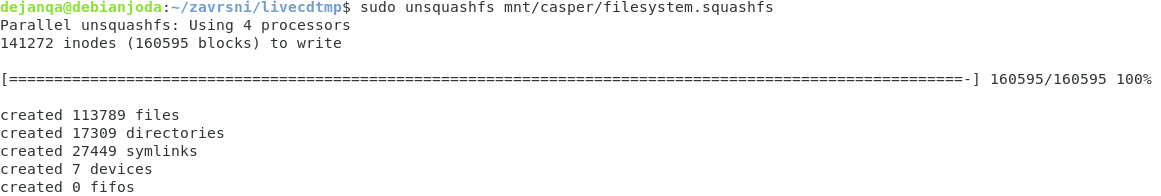
\includegraphics[width=\linewidth]{images/unsquashfscommand.png} 

\subsection*{Konfiguracija paketa za chroot okruženje}
\addcontentsline{toc}{subsection}{\numberline{}Konfiguracija paketa za chroot okruženje}
\noindent
Da bi imali mrežnu konekciju unutar edit-java direktorija jedno rješenje je kopirati /run direktorij unutar edit-java direktorija.
Najbolje manuelno popuniti resolv.conf unutar edit-java direktorija:
\begin{lstlisting}[style=BashInputStyle]
sudo gedit edit-java/etc/resolv.conf
\end{lstlisting}
Te unijeti sljedeći sadržaj i spasiti promjene:
(\textit{nameserver 1.1.1.1 \\
nameserver 8.8.8.8}).\\
\noindent
Isto važi i za etc/hosts datoteku:
\begin{lstlisting}[style=BashInputStyle]
sudo gedit edit-java/etc/hosts
\end{lstlisting}
Kopirati sadrzaj iz /etc/hosts datoteke na sistemu domacinu unutar edit-java/etc/hosts datoteke:
\begin{lstlisting}
127.0.0.1	localhost
127.0.1.1	debianjoda.joda.net	debianjoda
\end{lstlisting}

\noindent
Namjestiti edit-java/dev direktorij kopirajuci /dev/ direktorij sa hosta, zatim chroot u edit-java direktorij.
Obaviti mount instrukcije navedene ispod. Ukoliko korisnik odluči da obriše edit-java direktorij iz nekog razloga,
bilo bi potrebno uraditi unmount edit-java direktorija da sistem domaćin ne bi postao neupotrebljiv:
\begin{lstlisting}[style=BashInputStyle]
sudo mount --bind /dev/ edit-java/dev
sudo chroot edit-java
mount -t proc none /proc
mount -t sysfs none /sys
mount -t devpts none /dev/pts
\end{lstlisting}

\noindent
Takodjer potrebno je izvrsiti sljedece komande da bi se izbjegli problemi sa lokalizacijom:
\begin{lstlisting}[style=BashInputStyle]
export HOME=/root
export LC_ALL=C
\end{lstlisting}

\subsection*{Instalacija Java paketa unutar chroot okruženja}
\addcontentsline{toc}{subsection}{\numberline{}Instalacija Java paketa unutar chroot okruženja}
\noindent
Za ispis svih instaliranih paketa:
\begin{lstlisting}[style=BashInputStyle]
dpkg-query -W --showformat='\${Installed-Size}\t\${Package}\n' | sort -nr | less
\end{lstlisting}

\noindent
Instalacija java paketa:
\begin{lstlisting}[style=BashInputStyle]
apt update
apt install default-jdk
\end{lstlisting}
Provjera verzije java instalacije:
\begin{lstlisting}[style=BashInputStyle]
java -version
\end{lstlisting}
Rezultat prethodne komande bi trebao biti:
\begin{lstlisting}[style=BashInputStyle]
openjdk version "11.0.6" 2020-01-14
OpenJDK Runtime Environment (build 11.0.6+10-post-Ubuntu-1ubuntu118.04.1)
OpenJDK 64-Bit Server VM (build 11.0.6+10-post-Ubuntu-1ubuntu118.04.1, mixed mode, sharing)
\end{lstlisting}
Sada možemo instalirati Eclipse, koji je jedan od najpoznatijih JAVA IDE (Integrated Development Environment). Prvo ćemo preuzeti eclipse.tgz sa interneta pomoću wget komande, a zatim instalirati:
\begin{lstlisting}[style=BashInputStyle]
wget http://ftp.jaist.ac.jp/pub/eclipse/technology/epp/downloads/release/2019-03/R/eclipse-java-2019-03-R-linux-gtk-x86_64.tar.gz
tar -zxvf eclipse-java-2019-03-R-linux-gtk-x86_64.tar.gz -C /usr/
ln -s /usr/eclipse/eclipse /usr/bin/eclipse
nano /usr/share/applications/eclipse.desktop
\end{lstlisting}
Nakon posljednje komande unijeti sljedeći sadržaj:
\begin{lstlisting}[style=BashInputStyle]
[Desktop Entry]
Encoding=UTF-8
Name=Eclipse IDE
Comment=Eclipse IDE
Exec=/usr/bin/eclipse
Icon=/usr/eclipse/icon.xpm
Terminal=false
Type=Application
StartupNotify=false
\end{lstlisting}
Sada možemo pokrenuti eclipse međutim to ćemo kasnije uraditi kada pokrenemo iso file u kemu-kvm.
\noindent
Nakon završetka instalacije izvršiti unutar chroot:
\begin{lstlisting}[style=BashInputStyle]
apt clean
rm -rf /tmp/* ~/.bash_history
rm -rf /tmp/* ~/.bashrc
rm /var/lib/dbus/machine-id
rm /sbin/initctl
dpkg-divert --rename --remove /sbin/initctl
umount /proc || umount -lf /proc
umount /sys
umount /dev/pts
umount /dev
exit
\end{lstlisting}

\noindent
Ponovno generisati filesystem.manifest:
\begin{lstlisting}[style=BashInputStyle]
sudo chmod +w extract-java-cd/casper/filesystem.manifest
sudo su
chroot edit-java dpkg-query -W --showformat='${Package} ${Version}\n' > extract-java-cd/casper/filesystem.manifest
exit
sudo cp extract-java-cd/casper/filesystem.manifest extract-java-cd/casper/filesystem.manifest-desktop
sudo sed -i '/ubiquity/d' extract-java-cd/casper/filesystem.manifest-desktop
sudo sed -i '/casper/d' extract-java-cd/casper/filesystem.manifest-desktop
\end{lstlisting}

\subsection*{Generisanje filesystem.squashfs datoteke}
\addcontentsline{toc}{subsection}{\numberline{}Generisanje filesystem.squashfs datoteke}
\noindent
Sada cemo upotrijebiti drugu funkciju iz squashfs-tools, a to je mksquashfs. S tom funkcijom ćemo kompresovati edit-java direktorij u novu filesystem.squashfs datoteku, baš kao i u prethodna dva slučaja sa MongoDB i NodeJS modulima. U kodu ispod je potrebno izvršiti komandu iz linije 1 i jednu od preostale 3, pri čemu prva (komanda na liniji 2) daje najslabiju kompresiju, ali je najbrža. Druga komanda se duže izvršava ali je veći procenat kompresije u odnosu na prvu komandu. Dok je kod treće komande procenat kompresije najveći, a vrijeme izvršenja najduže:
\begin{lstlisting}[style=BashInputStyle]
sudo rm extract-java-cd/casper/filesystem.squashfs
sudo mksquashfs edit-java extract-java-cd/casper/filesystem.squashfs -nolzma 
sudo mksquashfs edit-java extract-java-cd/casper/filesystem.squashfs -b 1048576
sudo mksquashfs edit-java extract-java-cd/casper/filesystem.squashfs -comp xz -e edit/boot
\end{lstlisting}

\noindent
Naredni korak je da ažuriramo filesystem.size datoteku:
\begin{lstlisting}[style=BashInputStyle]
sudo su
printf $(du -sx --block-size=1 edit-java | cut -f1) > extract-java-cd/casper/filesystem.size
exit
\end{lstlisting}

\noindent
Nakon toga upisati naziv image-a unutar README.diskdefines. 
Upisati 'Ubuntu with Java 18.04.4 LTS "Bionic Beaver" - Release amd64' u polje DISKNAME:
\begin{lstlisting}[style=BashInputStyle]
sudo gedit extract-java-cd/README.diskdefines
\end{lstlisting}

\subsection*{Generisanje Ubuntu .iso image sa Java modulom}
\addcontentsline{toc}{subsection}{\numberline{}Generisanje Ubuntu .iso image sa Java modulom}
\noindent
Ažurirati md5sum.txt datoteku:
\begin{lstlisting}[style=BashInputStyle]
cd extract-java-cd
sudo rm md5sum.txt
find -type f -print0 | sudo xargs -0 md5sum | grep -v isolinux/boot.cat | sudo tee md5sum.txt
\end{lstlisting}

\noindent
Napokon možemo napraviti iso image koji će da sadrži Java modul. Za ovu operaciju koristimo funkciju genisoimage. Neke linux distribucije nude mkisofs funkciju. Tako da ukoliko ne radi genisoimage trebala bi raditi funkcija mkisofs:
\begin{lstlisting}[style=BashInputStyle]
sudo genisoimage -D -r -V "$IMAGE_NAME" -cache-inodes -J -l -b isolinux/isolinux.bin -c isolinux/boot.cat -no-emul-boot -boot-load-size 4 -boot-info-table -o ../ubuntu-with-java-18.04-amd64.iso .
\end{lstlisting}

\subsection*{Pokretanje iso image-a pomoću kvm biblioteke}
\addcontentsline{toc}{subsection}{\numberline{}Pokretanje iso image-a pomoću kvm biblioteke}
\indent
Sada ćemo napraviti virtuelni hard disk pomocu qemu-img komande da bismo pokrenuli na njemu naš novi modul Java Ubuntu.
\begin{lstlisting}[style=BashInputStyle]
cd ~
qemu-img create ubuntujava.img 5G
\end{lstlisting}

\noindent 
Pokrenućemo modul pomoću KVM-a:
\begin{lstlisting}[style=BashInputStyle]
sudo kvm -hda ubuntujava.img -cdrom ~/zavrsni/livecdtmp/ubuntu-with-java-18.04-amd64.iso -boot d -m 2048
\end{lstlisting}

\subsection*{Rezultat Modul Java}
\addcontentsline{toc}{subsection}{\numberline{}Rezultat Modul Java}
\indent
Slike ispod prikazuju verziju jave i Eclipse okruženje pokrenuto unutar KVM:
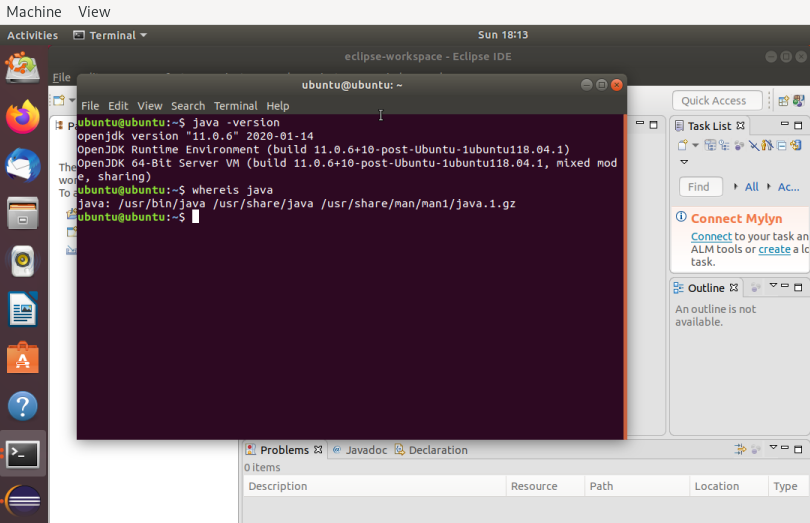
\includegraphics[width=\linewidth]{images/javaLive.png} 
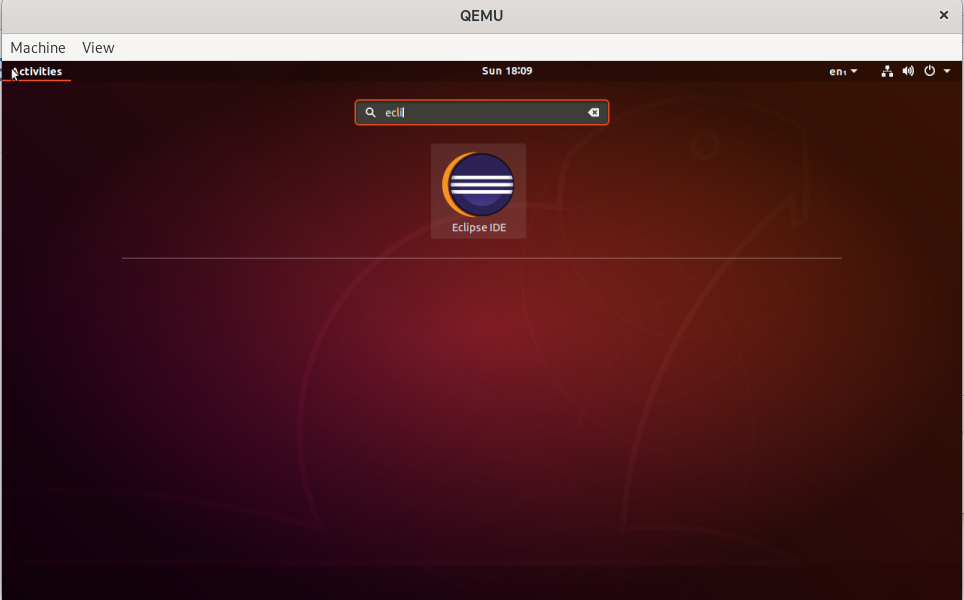
\includegraphics[width=\linewidth]{images/eclipseLive.png} 
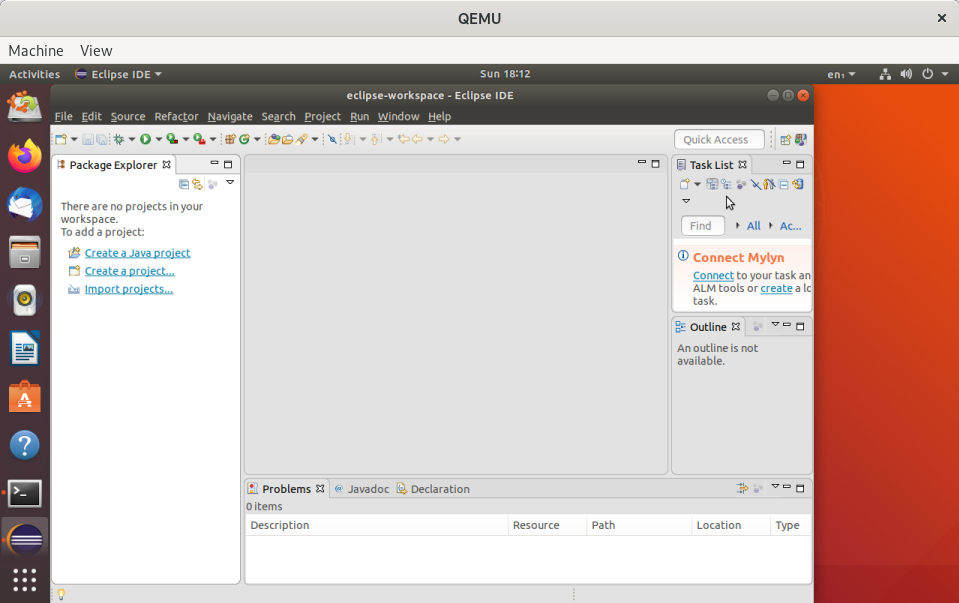
\includegraphics[width=\linewidth]{images/eclipseLive1.png} 
\newpage
\section*{Modul Chrome}
\addcontentsline{toc}{section}{\numberline{}Modul Chrome}
\indent
Kao treći primjer modularizacije squashfs datotečnog sistema, kreiran je modul Chrome. Kao što mu ime kaže, riječ je o modulu sa instaliranim Google Chrome pretraživačem. Većinom koraci su identični kao u prethodna 2 slučaja, izuzev koraka instaliranja dodatnih paketa unutar modula.\\
\indent
Google Chrome je mrežni pretraživač razvijen 2008. godine, prvo za Microsoft Windows, a kasnije i za Linux, MacOS, Android, iOS. Danas, 68\% od ukupnog broja pretraživača na desktop računarima su Google Chrome pretraživači. Sličan je procenat i kada su u pitanju mobilni uređaji.\\
\indent
Google Chrome je najpoznatiji web pretraživač vjerovatno zbog svoje brzine i jednostavnosti za povezivanje različitih uređaja putem Google korisničkog računa. Na većini Android uređaja Google Chrome dođe kao predinstaliran program. Glavne zasluge za dobre performanse Google Chrome pretraživača nosi Google V8 JavaScript virtuelna mašina, koju također koristi i NodeJS.
\subsection*{Kreiranje direktorija potrebnih za rad}
\addcontentsline{toc}{subsection}{\numberline{}Kreiranje direktorija potrebnih za rad}
\begin{lstlisting}[style=BashInputStyle]
cd ~/squashfs/livecdtmp
sudo mount -o loop ./isoimgs/ubuntu-18.04.4-desktop-amd64.iso mnt
mkdir extract-chrome-cd
sudo rsync --exclude=/casper/filesystem.squashfs -a mnt/ extract-chrome-cd
mkdir modul-chrome
sudo rsync -a extract-chrome-cd/ modul-chrome
\end{lstlisting}

\subsection*{unsquashfs filesystem.squashs datoteke}
\addcontentsline{toc}{subsection}{\numberline{}unsquashfs filesystem.squashfs datoteke}

Zatim slijedi korak u kojem se opet raspakuje filesystem.squashfs direktorij i kopiramo ga u edit-chrome direktorij. Ovaj put ćemo edit direktorij imenovati edit-chrome da ne izgubimo prethodni sadržaj edit direktorija.\\
\begin{lstlisting}[style=BashInputStyle]
sudo unsquashfs mnt/casper/filesystem.squashfs
sudo mv squashfs-root/ edit-chrome
\end{lstlisting}

\subsection*{Konfiguracija paketa za chroot okruženje}
\addcontentsline{toc}{subsection}{\numberline{}Konfiguracija paketa za chroot okruženje}
\indent
Da bi imali mrežnu konekciju unutar edit-chrome direktorija jedno rješenje je kopirati /run direktorij unutar edit-chrome direktorija.
Najbolje manuelno popuniti resolv.conf unutar edit-chrome direktorija: \\
\begin{lstlisting}[style=BashInputStyle]
sudo gedit edit-chrome/etc/resolv.conf
\end{lstlisting}
\textit{nameserver 1.1.1.1 \\
nameserver 8.8.8.8}\\
Isto važi i za etc/hosts datoteku. Najbolje je provjeriti nakon izvršenih komandi da li je upisan sadržaj u resolv.conf i hosts datoteke, te ukoliko nije dopuniti nedostatke:
\noindent
Isto važi i za etc/hosts datoteku:
\begin{lstlisting}[style=BashInputStyle]
sudo gedit edit-chrome/etc/hosts
\end{lstlisting}
Kopirati sadržaj iz /etc/hosts datoteke na sistemu domaćinu unutar edit-chrome/etc/hosts datoteke:
\begin{lstlisting}
127.0.0.1	localhost
127.0.1.1	debianjoda.joda.net	debianjoda
\end{lstlisting}

\noindent
Namjestiti edit-chrome/dev direktorij kopirajući /dev/ direktorij sa hosta, zatim chroot u edit-chrome direktorij.
Obaviti mount instrukcije navedene ispod. Ukoliko korisnik odluči da obriše edit-chrome direktorij iz nekog razloga,
bilo bi potrebno uraditi unmount edit-chrome direktorija da sistem domaćin ne bi postao neupotrebljiv:
\begin{lstlisting}[style=BashInputStyle]
sudo mount --bind /dev/ edit-chrome/dev
sudo chroot edit-chrome
mount -t proc none /proc
mount -t sysfs none /sys
mount -t devpts none /dev/pts
\end{lstlisting}

Također potrebno je izvršiti sljedeće komande da bi se izbjegli problemi sa lokalizacijom:
\begin{lstlisting}[style=BashInputStyle]
export HOME=/root
export LC_ALL=C
\end{lstlisting}

\subsection*{Instalacija Google Chrome paketa unutar chroot okruženja}
\addcontentsline{toc}{subsection}{\numberline{}Instalacija Google Chrome paketa unutar chroot okruženja}
\noindent
Za ispis svih instaliranih paketa:
\begin{lstlisting}[style=BashInputStyle]
dpkg-query -W --showformat='\${Installed-Size}\t\${Package}\n' | sort -nr | less
\end{lstlisting}

\noindent
Instalacija google-chrome paketa:
\begin{lstlisting}[style=BashInputStyle]
sudo nano /etc/apt/sources.list.d/google-chrome.list
\end{lstlisting}
Te upisati u ovu datoteku sljedeći sadržaj
\begin{lstlisting}[style=BashInputStyle]
deb [arch=amd64] http://dl.google.com/linux/chrome/deb/ stable main
\end{lstlisting}
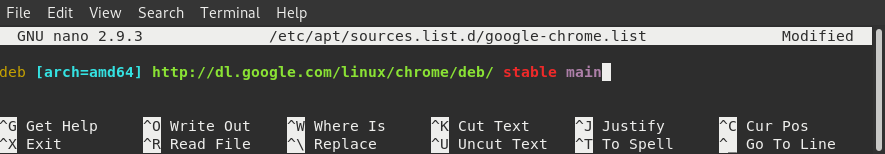
\includegraphics[width=\linewidth]{images/google-chrome-list.png} 

Zatim spasiti datoteku unutar nano editora sa \textbf{CTRL+O}, \textbf{ENTER} za potvrdu i \textbf{CTRL+X} za izlaz iz nano editora.\\
Sljedeća komanda preuzima Google javni ključ da bismo mogli instalirati google-chrome. Zatim komandom apt-key dodajemo ključ u prsten javnih ključeva da bi apt mogao potvrditi integritet Google Chrome paketa.\\
\begin{lstlisting}[style=BashInputStyle]
wget https://dl.google.com/linux/linux_signing_key.pub
sudo apt-key add linux_signing_key.pub
\end{lstlisting}
Trebao bi izlaz prethodne komande biti "OK".\\
\indent
Sada izvršimo ažuriranje liste paketa i instaliramo google-chrome-stable paket:
\begin{lstlisting}[style=BashInputStyle]
apt update
apt install google-chrome-stable
\end{lstlisting}

Provjera instalacije:
\begin{lstlisting}[style=BashInputStyle]
google-chrome-stable --version
\end{lstlisting}
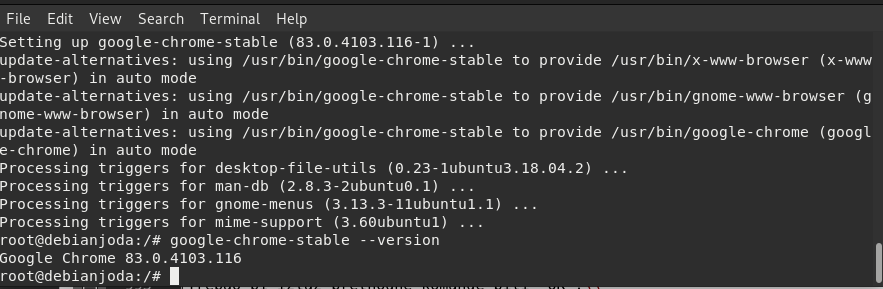
\includegraphics[width=\linewidth]{images/googlechromestableversion.png} 

\noindent
Nakon završetka instalacije izvršiti unutar chroot:
\begin{lstlisting}[style=BashInputStyle]
apt clean
rm -rf /tmp/* ~/.bash_history
rm -rf /tmp/* ~/.bashrc
rm /var/lib/dbus/machine-id
rm /sbin/initctl
dpkg-divert --rename --remove /sbin/initctl
umount /proc || umount -lf /proc
umount /sys
umount /dev/pts
umount /dev
exit
\end{lstlisting}

\noindent
Ponovno generisati filesystem.manifest:
\begin{lstlisting}[style=BashInputStyle]
sudo chmod +w extract-chrome-cd/casper/filesystem.manifest
sudo su
chroot edit-chrome dpkg-query -W --showformat='${Package} ${Version}\n' > extract-chrome-cd/casper/filesystem.manifest
exit
sudo cp extract-chrome-cd/casper/filesystem.manifest extract-chrome-cd/casper/filesystem.manifest-desktop
sudo sed -i '/ubiquity/d' extract-chrome-cd/casper/filesystem.manifest-desktop
sudo sed -i '/casper/d' extract-chrome-cd/casper/filesystem.manifest-desktop
sudo umount edit-chrome/dev
\end{lstlisting}

\subsection*{Generisanje filesystem.squashfs datoteke}
\addcontentsline{toc}{subsection}{\numberline{}Generisanje filesystem.squashfs datoteke}
\noindent
Sada ćemo upotrijebiti drugu funkciju iz squashfs-tools, a to je mksquashfs. S tom funkcijom ćemo kompresovati edit-chrome direktorij u novu filesystem.squashfs datoteku. U kodu ispod je potrebno izvršiti komandu iz linije 1 i jednu od preostale 3, pri čemu prva (komanda na liniji 2) daje najslabiju kompresiju, ali je najbrža. Druga komanda se duže izvršava ali je veći procenat kompresije u odnosu na prvu komandu. Dok je kod treće komande procenat kompresije najveći, a vrijeme izvršenja najduže:
\begin{lstlisting}[style=BashInputStyle]
sudo rm extract-chrome-cd/casper/filesystem.squashfs
sudo mksquashfs edit-chrome extract-chrome-cd/casper/filesystem.squashfs -nolzma 
sudo mksquashfs edit-chrome extract-chrome-cd/casper/filesystem.squashfs -b 1048576
sudo mksquashfs edit-chrome extract-chrome-cd/casper/filesystem.squashfs -comp xz -e edit/boot
\end{lstlisting}

\noindent
Naredni korak je da ažuriramo filesystem.size datoteku:
\begin{lstlisting}[style=BashInputStyle]
sudo su
printf $(du -sx --block-size=1 edit-chrome | cut -f1) > extract-chrome-cd/casper/filesystem.size
exit
\end{lstlisting}

\noindent
Nakon toga upisati naziv image-a unutar README.diskdefines. 
Upisati 'Ubuntu with Google Chrome 18.04.4 LTS "Bionic Beaver" - Release amd64' u polje DISKNAME:
\begin{lstlisting}[style=BashInputStyle]
sudo gedit extract-chrome-cd/README.diskdefines
\end{lstlisting}

\subsection*{Generisanje Ubuntu .iso image sa Google Chrome modulom}
\addcontentsline{toc}{subsection}{\numberline{}Generisanje Ubuntu .iso image sa Google Chrome modulom}
\noindent
Ažurirati md5sum.txt datoteku:
\begin{lstlisting}[style=BashInputStyle]
cd extract-chrome-cd
sudo rm md5sum.txt
find -type f -print0 | sudo xargs -0 md5sum | grep -v isolinux/boot.cat | sudo tee md5sum.txt
\end{lstlisting}

\noindent
Napokon možemo napraviti iso image koji će da sadrži Google Chrome modul. Za ovu operaciju koristimo funkciju genisoimage. Neke linux distribucije nude mkisofs funkciju. Tako da ukoliko ne radi genisoimage trebala bi raditi funkcija mkisofs:
\begin{lstlisting}[style=BashInputStyle]
sudo genisoimage -D -r -V "$IMAGE_NAME" -cache-inodes -J -l -b isolinux/isolinux.bin -c isolinux/boot.cat -no-emul-boot -boot-load-size 4 -boot-info-table -o ../ubuntu-with-chrome-18.04-amd64.iso .
\end{lstlisting}

\subsection*{Pokretanje iso image-a pomoću kvm biblioteke}
\addcontentsline{toc}{subsection}{\numberline{}Pokretanje iso image-a pomoću kvm biblioteke}
\indent
Sada ćemo napraviti virtuelni hard disk pomoću qemu-img komande da bismo pokrenuli na njemu naš novi modul Google Chrome Ubuntu.
\begin{lstlisting}[style=BashInputStyle]
cd ~
qemu-img create ubuntuchrome.img 5G
\end{lstlisting}

\noindent 
Pokrenućemo modul pomoću KVM-a:
\begin{lstlisting}[style=BashInputStyle]
sudo kvm -hda ubuntuchrome.img -cdrom ~/zavrsni/livecdtmp/ubuntu-with-chrome-18.04-amd64.iso -boot d -m 2048
\end{lstlisting}

\subsection*{Rezultat Modul Chrome}
\addcontentsline{toc}{subsection}{\numberline{}Rezultat Modul Chrome}
\indent
Nakon što se pokrene naš sistem u QEMU, odaberemo opciju Try Ubuntu. Možemo se uvjeriti da je Google Chrome instaliran, što pokazuju slike ispod:\\
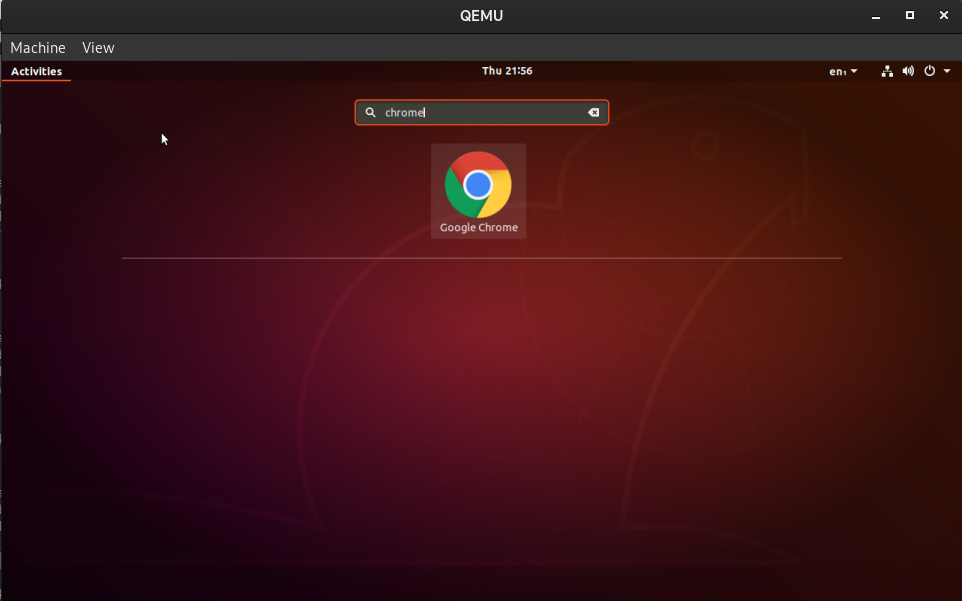
\includegraphics[width=\linewidth]{images/chromeLive.png}\\\\
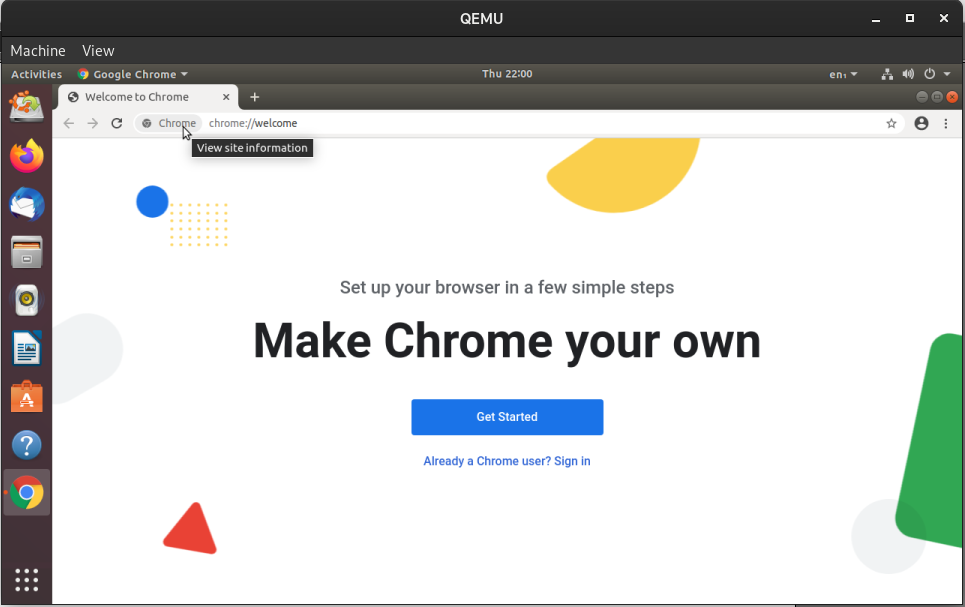
\includegraphics[width=\linewidth]{images/chromeLive2.png}\\

\chapter*{Kreiranje više modula unutar jedne .iso datoteke}
\addcontentsline{toc}{chapter}{\numberline{}Kreiranje više modula unutar jedne .iso datoteke}
\indent
U prethodnom dijelu rada je opisan proces kreiranja zasebnih .iso datoteka za svaki od modula. Sada će biti opisan proces kreiranja modularne .iso datoteke u kojoj će postojati opcija aktivacije i deaktivacije pojedinih modula.\\
Ovakav pristup podrazumijeva više filesystem.squashfs datoteka unutar jedne .iso datoteke. Cilj je da se kreira jedan bazni modul koji će sadržavati baznu filesystem.squashfs datoteku i ostale *.squashfs datoteke od pojedinih modula. Ova bazna filesystem.squashfs datoteka bi jedina trebala biti kompletna squashfs datoteka. Ostale squasfhfs datoteke bi samo trebale sadržavati razlike između edit datotečnih sistema pojedinih modula sa baznim datotečnim sistemom.\\
Delta funkcije će se raditi naspram edit direktorija a sve *.squashfs datoteke će naposljetku biti smještene u bazni-modul direktorij.
\indent
Razlika izmedju edit direktorija pojedinih modula sa baznim edit direktorijem bi bile datoteke instaliranih paketa, kao što su java paketi, nodejs paketi, google-chrome paketi i mongodb paketi. Pored ovih razlika postoji i jedna bitna datoteka koja će se razlikovati, a to je /var/lib/dpkg/status datoteka. Ona sadrži popis svih instaliranih paketa. Za svaki modul bismo trebali napraviti delta direktorij koji sadrži razlike između baznog edit direktorija sa novokreiranim  edit direktorijem pojedinog modula. Također unutar delta direktorija bismo kreirali status.diff datoteku koja sadrži razliku status datoteke baznog edit direktorija i status datoteke edit direktorija novog modula.\\
\indent
Deaktivacija pojedinog modula bi podrazumijevala izvršavanje umount komande tog modula. Kao i ponovno generisanje status datoteke pri čemu bi nova status datoteka bila razlika između bazne status datoteke i status.diff datoteke tog modula.

\section*{Bazni modul}
\addcontentsline{toc}{section}{\numberline{}Bazni modul}
\indent
Direktorij bazni-modul će biti naš odredišni direktorij koji će da sadrži sve .squashfs datoteke. Od njega ćemo na posljetku generisati .iso datoteku koja će da sadrži sve module, za razliku od pristupa opisanog u prethodnom poglavlju gdje su generisane 4 zasebne iso datoteke za svaki modul po jedna.\\
Ispočetka ćemo generisati bazni-modul direktorij koji je raspakovana ubuntu-18.04.4-desktop-amd64.iso datoteka sa izmjenama u etc/hosts i etc/resolv.conf datotekama. Izmjene u ove dvije datoteke su nam potrebne da bismo unutar KVM-a pri pokretanju naše .iso datoteke imali mrežnu konekciju.\\
Prvi korak nam je da montiramo ubuntu-18.04.4-desktop-amd64.iso datoteku na mnt direktorij:
\begin{lstlisting}[style=BashInputStyle]
sudo mount -o loop ./isoimgs/ubuntu-18.04.4-desktop-amd64.iso mnt
\end{lstlisting}

Zatim napravimo direktorij pod nazivom bazni-modul u kojeg ćemo kopirati mnt direktorij izostavljajući filesystem.squashfs datoteku unutar /casper direktorija:
\begin{lstlisting}[style=BashInputStyle]
mkdir bazni-modul
sudo rsync --exclude=/casper/filesystem.squashfs -a mnt/ bazni-modul
\end{lstlisting}

Napomena da smo izostavili filesystem.squashfs datoteke jer ćemo generisati nove .squashfs datoteke koje će biti pozicionirane u /casper direktorij bazni-modul direktorija.

\section*{Bazni edit}
\addcontentsline{toc}{section}{\numberline{}Bazni edit}
\indent
Slijedi korak u kojem koristeći unsquashfs funkciju raspakujemo kompresovanu filesystem.squashfs datoteku te kopiramo taj raspakovani sadržaj u direktorij pod nazivom bazni-edit. Unutar ovog direktorija ćemo podesiti opće mrežne postavke u hosts i resolv.conf datotekama.
\begin{lstlisting}[style=BashInputStyle]
sudo unsquashfs mnt/casper/filesystem.squashfs
sudo mv squashfs-root/ bazni-edit
\end{lstlisting}

Sada ćemo u bazni-edit/etc direktoriju modifikovati datoteke hosts i resolv.conf:
\begin{lstlisting}[style=BashInputStyle]
sudo gedit bazni-edit/etc/resolv.conf
\end{lstlisting}
Te unijeti sljedeći sadržaj i spasiti promjene:
(\textit{nameserver 1.1.1.1 \\
nameserver 8.8.8.8}).\\
\noindent
Modifikacija etc/hosts datoteke:
\begin{lstlisting}[style=BashInputStyle]
sudo gedit bazni-edit/etc/hosts
\end{lstlisting}
Kopirati sadržaj iz /etc/hosts datoteke na sistemu domaćinu unutar bazni-edit/etc/hosts datoteke. U mom konkretnom slučaju to je sljedeći sadržaj:
\begin{lstlisting}
127.0.0.1	localhost
127.0.1.1	debianjoda.joda.net	debianjoda
\end{lstlisting}

\noindent
Još nam ostaje podešavanje bazni-edit/dev direktorija. To ćemo postići kao i u prethodnim koracima gdje smo pravili zasebne iso image-e od pojedinih modula, kopirajući /dev/ direktorij sa hosta, zatim chroot u bazni-edit direktorij, te izvršavanje mount instrukcija navedenih ispod:
\begin{lstlisting}[style=BashInputStyle]
sudo mount --bind /dev/ bazni-edit/dev
sudo chroot bazni-edit
mount -t proc none /proc
mount -t sysfs none /sys
mount -t devpts none /dev/pts
\end{lstlisting}

\noindent
Također potrebno je izvršiti sljedeće komande da bi se izbjegli problemi sa lokalizacijom:
\begin{lstlisting}[style=BashInputStyle]
export HOME=/root
export LC_ALL=C
\end{lstlisting}

Potom ćemo izvršiti čišćenje unutar chroot okruženja te komandom exit izaći iz chroot okruženja:
\begin{lstlisting}[style=BashInputStyle]
apt-get clean
rm -rf /tmp/* ~/.bash_history
rm -rf /tmp/* ~/.bashrc
rm /var/lib/dbus/machine-id
rm /sbin/initctl
dpkg-divert --rename --remove /sbin/initctl
umount /proc || umount -lf /proc
umount /sys
umount /dev/pts
umount /dev
exit
\end{lstlisting}
\indent
U ovom trenutku imamo bazni-edit direktorij. Iz njega ćemo sada napraviti edit direktorije ostalih modula. Napomena da će se u nastavku procesa također ponavljati većina komandi koje su potrebne za izvršenje, uz razlike u nazivima direktorija. Svakako je primjetno da su i u prethodnom dijelu rada također komande više puta ponovljene za iste dijelova procesa za pojedine module. Ali činjenica je da je proces dosta repetitivan.

\section*{NodeJS edit}
\addcontentsline{toc}{section}{\numberline{}NodeJS edit}

\indent
Sljedećom komandom ćemo kopirati bazni-edit direktorij u nodejs-edit direktorij:
\begin{lstlisting}[style=BashInputStyle]
mkdir nodejs-edit
sudo rsync -a bazni-edit/ nodejs-edit
\end{lstlisting}

Sada ćemo montirati /dev/ direktorij na nodejs-edit/dev putanju, te chroot u nodejs-edit direktorij. Potom slijede 3 mount komande korištene i u prethodnim slučajevima modifikacije unutar chroot okruženja:
\begin{lstlisting}[style=BashInputStyle]
sudo mount --bind /dev/ nodejs-edit/dev
sudo chroot nodejs-edit
mount -t proc none /proc
mount -t sysfs none /sys
mount -t devpts none /dev/pts
\end{lstlisting}

Za svaki slučaj ćemo podesiti sljedeće sistemske varijable:
\begin{lstlisting}[style=BashInputStyle]
export HOME=/root
export LC_ALL=C
\end{lstlisting}

Instalacija nodejs paketa:
\begin{lstlisting}[style=BashInputStyle]
apt-get update
apt-get install curl
curl -sL https://deb.nodesource.com/setup_13.x | sudo -E bash -
apt-get install -y nodejs
\end{lstlisting}

Tako je instaliran nodejs što može biti provjereno sljedećom komandom:
\begin{lstlisting}[style=BashInputStyle]
node --version
\end{lstlisting}

\noindent
Nakon završetka instalacije izvršiti unutar chroot:
\begin{lstlisting}[style=BashInputStyle]
apt-get clean
rm -rf /tmp/* ~/.bash_history
rm -rf /tmp/* ~/.bashrc
rm /var/lib/dbus/machine-id
rm /sbin/initctl
dpkg-divert --rename --remove /sbin/initctl
umount /proc || umount -lf /proc
umount /sys
umount /dev/pts
umount /dev
exit
\end{lstlisting}

Sada je dovršen i nodejs-edit direktorij. Njega ćemo uprijebiti za poređenje sa bazni-edit direktorijem da bismo dobili deltu između 2 direktorija. Od delta direktorija će se praviti nodejs.squashfs datoteka koju ćemo kopirati u bazni-modul/casper direktorij.

\section*{MongoDB edit}
\addcontentsline{toc}{section}{\numberline{}MongoDB edit}

\indent
Sljedećom komandom ćemo kopirati bazni-edit direktorij u mongodb-edit direktorij:
\begin{lstlisting}[style=BashInputStyle]
mkdir mongodb-edit
sudo rsync -a bazni-edit/ mongodb-edit
\end{lstlisting}

Sada ćemo montirati /dev/ direktorij na mongodb-edit/dev putanju, te chroot u mongodb-edit direktorij. Potom slijede 3 mount komande korištene i u prethodnim slučajevima modifikacije unutar chroot okruženja:
\begin{lstlisting}[style=BashInputStyle]
sudo mount --bind /dev/ mongodb-edit/dev
sudo chroot mongodb-edit
mount -t proc none /proc
mount -t sysfs none /sys
mount -t devpts none /dev/pts
\end{lstlisting}

Podesit ćemo i sistemske varijable:
\begin{lstlisting}[style=BashInputStyle]
export HOME=/root
export LC_ALL=C
\end{lstlisting}

\noindent
Da bismo mogli pokrenuti mongoDB, neophodno je instalirati libcurl4 i openssl pakete:
\begin{lstlisting}[style=BashInputStyle]
apt-get update
apt-get install libcurl4 openssl
\end{lstlisting}
Preuzimanje mongodb paketa sa interneta:
\begin{lstlisting}[style=BashInputStyle]
wget https://fastdl.mongodb.org/linux/mongodb-linux-x86_64-ubuntu1804-4.2.5.tgz
\end{lstlisting}
Ekstrakcija paketa:
\begin{lstlisting}[style=BashInputStyle]
tar -zxvf mongodb-linux-x86_64-ubuntu1804-4.2.5.tgz
\end{lstlisting}
Da bismo izbjegli potrebu da postavimo putanju u PATH sistemsku varijablu, kopiraćemo mongodb bin direktorij u /usr/local/bin/ direktorij:
\begin{lstlisting}[style=BashInputStyle]
cp mongodb-linux-x86_64-ubuntu1804-4.2.5/bin/* /usr/local/bin/
\end{lstlisting}
Konfiguracija mongodb paketa:\\
Prvo napravimo direktorij u koji će mongodb spremati podatke:
\begin{lstlisting}[style=BashInputStyle]
mkdir -p /var/lib/mongo
\end{lstlisting}
Također potrebno je napraviti direktorij u koji će se spremat logovi:
\begin{lstlisting}[style=BashInputStyle]
mkdir -p /var/log/mongodb
\end{lstlisting}
Potrebno je ažurirati privilegije pristupa na novokreirane direktorije:
\begin{lstlisting}[style=BashInputStyle]
chown `whoami` /var/lib/mongo 
chown `whoami` /var/log/mongodb
\end{lstlisting}
Sada možemo pokrenuti mongod proces:
\begin{lstlisting}[style=BashInputStyle]
mongod --dbpath /var/lib/mongo --logpath /var/log/mongodb/mongod.log --fork
\end{lstlisting}
Provjera instalacije:
\begin{lstlisting}[style=BashInputStyle]
mongo --version
\end{lstlisting}
Rezultat komande bi trebao potvrditi uspješno instaliran mongodb:
\begin{lstlisting}[style=BashInputStyle]
MongoDB shell version v4.2.5
git version: 2261279b51ea13df08ae708ff278f0679c59dc32
OpenSSL version: OpenSSL 1.1.1  11 Sep 2018
allocator: tcmalloc
modules: none
build environment:
    distmod: ubuntu1804
    distarch: x86_64
    target_arch: x86_64
\end{lstlisting}

\noindent
Nakon završetka instalacije izvršiti unutar chroot "čišćenje":
\begin{lstlisting}[style=BashInputStyle]
apt-get clean
rm -rf /tmp/* ~/.bash_history
rm -rf /tmp/* ~/.bashrc
rm /var/lib/dbus/machine-id
rm /sbin/initctl
dpkg-divert --rename --remove /sbin/initctl
umount /proc || umount -lf /proc
umount /sys
umount /dev/pts
umount /dev
exit
\end{lstlisting}

Tako je dovršen proces kreiranja mongodb-edit direktorija. On će biti upotrijebljen za poređenje sa bazni-edit direktorijem. Od tog delta direktorija će biti stvorena mongodb.squashfs datoteka.

\section*{Java edit}
\addcontentsline{toc}{section}{\numberline{}Java edit}

\indent
Sljedećom komandom ćemo kopirati bazni-edit direktorij u java-edit direktorij:
\begin{lstlisting}[style=BashInputStyle]
mkdir java-edit
sudo rsync -a bazni-edit/ java-edit
\end{lstlisting}

Sada ćemo montirati /dev/ direktorij na java-edit/dev putanju, te chroot u java-edit direktorij. Potom slijede 3 mount komande korištene i u prethodnim slučajevima modifikacije unutar chroot okruženja:
\begin{lstlisting}[style=BashInputStyle]
sudo mount --bind /dev/ java-edit/dev
sudo chroot java-edit
mount -t proc none /proc
mount -t sysfs none /sys
mount -t devpts none /dev/pts
\end{lstlisting}

Podesit ćemo i sistemske varijable:
\begin{lstlisting}[style=BashInputStyle]
export HOME=/root
export LC_ALL=C
\end{lstlisting}

\noindent
Instalacija java paketa:
\begin{lstlisting}[style=BashInputStyle]
apt update
apt install default-jdk
\end{lstlisting}
Provjera verzije java instalacije:
\begin{lstlisting}[style=BashInputStyle]
java -version
\end{lstlisting}
Rezultat prethodne komande bi trebao biti:
\begin{lstlisting}[style=BashInputStyle]
openjdk version "11.0.8" 2020-07-14
OpenJDK Runtime Environment (build 11.0.8+10-post-Ubuntu-0ubuntu118.04.1)
OpenJDK 64-Bit Server VM (build 11.0.8+10-post-Ubuntu-0ubuntu118.04.1, mixed mode, sharing)
\end{lstlisting}
Sada možemo instalirati Eclipse, koji je već spomenut u prethodnom odjeljku Modul Java. Prvo ćemo preuzeti eclipse.tgz sa interneta pomoću wget komande, a zatim instalirati:
\begin{lstlisting}[style=BashInputStyle]
wget http://ftp.jaist.ac.jp/pub/eclipse/technology/epp/downloads/release/2019-03/R/eclipse-java-2019-03-R-linux-gtk-x86_64.tar.gz
tar -zxvf eclipse-java-2019-03-R-linux-gtk-x86_64.tar.gz -C /usr/
ln -s /usr/eclipse/eclipse /usr/bin/eclipse
nano /usr/share/applications/eclipse.desktop
\end{lstlisting}
Nakon posljednje komande unijeti sljedeći sadržaj:
\begin{lstlisting}[style=BashInputStyle]
[Desktop Entry]
Encoding=UTF-8
Name=Eclipse IDE
Comment=Eclipse IDE
Exec=/usr/bin/eclipse
Icon=/usr/eclipse/icon.xpm
Terminal=false
Type=Application
StartupNotify=false
\end{lstlisting}

\noindent
Nakon završetka instalacije izvršiti unutar chroot:
\begin{lstlisting}[style=BashInputStyle]
apt clean
rm -rf /tmp/* ~/.bash_history
rm -rf /tmp/* ~/.bashrc
rm /var/lib/dbus/machine-id
rm /sbin/initctl
dpkg-divert --rename --remove /sbin/initctl
umount /proc || umount -lf /proc
umount /sys
umount /dev/pts
umount /dev
exit
\end{lstlisting}

\section*{Chrome edit}
\addcontentsline{toc}{section}{\numberline{}Chrome edit}

\indent
Sljedećom komandom ćemo kopirati bazni-edit direktorij u chrome-edit direktorij:
\begin{lstlisting}[style=BashInputStyle]
mkdir chrome-edit
sudo rsync -a bazni-edit/ chrome-edit
\end{lstlisting}

Sada ćemo montirati /dev/ direktorij na chrome-edit/dev putanju, te chroot u chrome-edit direktorij. Potom slijede 3 mount komande korištene i u prethodnim slučajevima modifikacije unutar chroot okruženja:
\begin{lstlisting}[style=BashInputStyle]
sudo mount --bind /dev/ chrome-edit/dev
sudo chroot chrome-edit
mount -t proc none /proc
mount -t sysfs none /sys
mount -t devpts none /dev/pts
\end{lstlisting}

Podesit ćemo i sistemske varijable:
\begin{lstlisting}[style=BashInputStyle]
export HOME=/root
export LC_ALL=C
\end{lstlisting}

\noindent
Instalacija google-chrome paketa:
\begin{lstlisting}[style=BashInputStyle]
sudo nano /etc/apt/sources.list.d/google-chrome.list
\end{lstlisting}
Te upisati u ovu datoteku sljedeći sadržaj
\begin{lstlisting}[style=BashInputStyle]
deb [arch=amd64] http://dl.google.com/linux/chrome/deb/ stable main
\end{lstlisting}
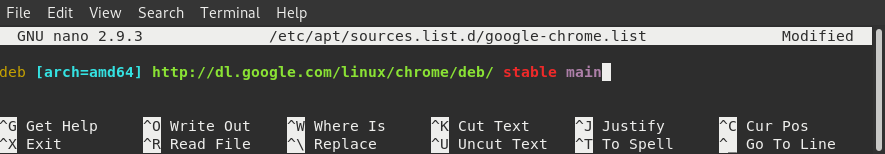
\includegraphics[width=\linewidth]{images/google-chrome-list.png} 

Zatim spasiti datoteku unutar nano editora sa \textbf{CTRL+O}, \textbf{ENTER} za potvrdu i \textbf{CTRL+X} za izlaz iz nano editora.\\
Sljedeća komanda preuzima Google javni ključ da bismo mogli instalirati google-chrome. Zatim komandom apt-key dodajemo ključ u prsten javnih ključeva da bi apt mogao potvrditi integritet Google Chrome paketa.\\
\begin{lstlisting}[style=BashInputStyle]
wget https://dl.google.com/linux/linux_signing_key.pub
sudo apt-key add linux_signing_key.pub
\end{lstlisting}
Trebao bi izlaz prethodne komande biti "OK".\\
\indent
Sada izvršimo ažuriranje liste paketa i instaliramo google-chrome-stable paket:
\begin{lstlisting}[style=BashInputStyle]
apt update
apt install google-chrome-stable
\end{lstlisting}

Provjera instalacije:
\begin{lstlisting}[style=BashInputStyle]
google-chrome-stable --version
\end{lstlisting}
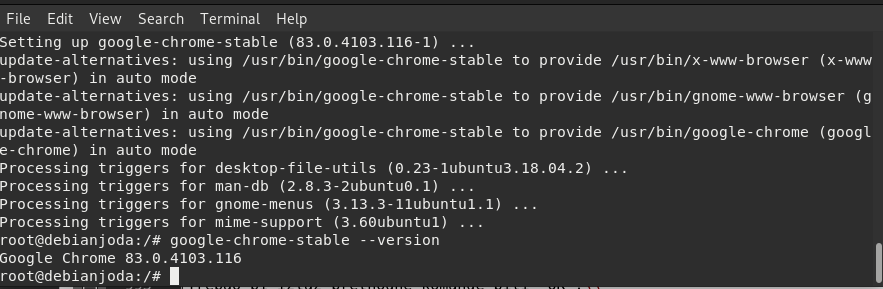
\includegraphics[width=\linewidth]{images/googlechromestableversion.png} 

\noindent
Nakon završetka instalacije izvršiti unutar chroot:
\begin{lstlisting}[style=BashInputStyle]
apt clean
rm -rf /tmp/* ~/.bash_history
rm -rf /tmp/* ~/.bashrc
rm /var/lib/dbus/machine-id
rm /sbin/initctl
dpkg-divert --rename --remove /sbin/initctl
umount /proc || umount -lf /proc
umount /sys
umount /dev/pts
umount /dev
exit
\end{lstlisting}

Tako je kreiran chrome-edit direktorij. Njega ćemo kao i prethodne edit direktorije uporediti sa bazni-edit direktorijem da bismo dobili delta direktorij. Od delta direktorija će se kreirati chrome.squashfs datoteka koju ćemo pozicionirati u bazni-modul/casper direktoriju kao i ostale .squashfs datoteke.

\section*{Generisanje bazne filesystem.squashfs datoteke}
\addcontentsline{toc}{section}{\numberline{}Generisanje bazne filesystem.squashfs datoteke}
\indent
Prvo ćemo nanovo generisati filesystem.manifest:
\begin{lstlisting}[style=BashInputStyle]
sudo chmod +w bazni-modul/casper/filesystem.manifest
sudo su
chroot bazni-edit dpkg-query -W --showformat='${Package} ${Version}\n' > bazni-modul/casper/filesystem.manifest
exit
sudo cp bazni-modul/casper/filesystem.manifest bazni-modul/casper/filesystem.manifest-desktop
sudo sed -i '/ubiquity/d' bazni-modul/casper/filesystem.manifest-desktop
sudo sed -i '/casper/d' bazni-modul/casper/filesystem.manifest-desktop
\end{lstlisting}

\noindent
Sada ćemo upotrijebiti funkciju mksquashfs iz squashfs-tools. S tom funkcijom ćemo kompresovati bazni-edit direktorij u novu filesystem.squashfs datoteku. U kodu ispod je potrebno izvršiti komandu iz linije 1 i jednu od preostale 3, pri čemu prva (komanda na liniji 2) daje najslabiju kompresiju, ali je najbrža. Druga komanda se duže izvršava ali je veći procenat kompresije u odnosu na prvu komandu. Dok je kod treće komande procenat kompresije najveći, a vrijeme izvršenja najduže:
\begin{lstlisting}[style=BashInputStyle]
sudo rm bazni-modul/casper/filesystem.squashfs
sudo mksquashfs bazni-edit bazni-modul/casper/filesystem.squashfs -nolzma 
sudo mksquashfs bazni-edit bazni-modul/casper/filesystem.squashfs -b 1048576
sudo mksquashfs bazni-edit bazni-modul/casper/filesystem.squashfs -comp xz -e edit/boot
\end{lstlisting}

\noindent
Naredni korak je da ažuriramo filesystem.size datoteku:
\begin{lstlisting}[style=BashInputStyle]
sudo su
printf $(du -sx --block-size=1 bazni-edit | cut -f1) > bazni-modul/casper/filesystem.size
exit
\end{lstlisting}

\section*{Generisanje nodejs.squashfs datoteke}
\addcontentsline{toc}{section}{\numberline{}Generisanje nodejs.squashfs datoteke}
\indent
Proces kreiranja nodejs.squashfs datoteke će zahtijevati prije svega generisanje delta direktorija koji sadrži sve razlike između bazni-edit i nodejs-edit direktorija. Također se podrazumijeva kreiranje status.diff datoteke koja će sadržati razliku između status datoteka bazni-edit i nodejs-edit direktorija.\\

\subsection*{Kreiranje nodejsBazniDelta direktorija}
\addcontentsline{toc}{subsection}{\numberline{}Kreiranje nodejsBazniDelta direktorija}
\begin{lstlisting}[style=BashInputStyle]
mkdir nodejsBazniDelta
sudo rsync -rvcm --compare-dest=/home/user/zavrsni/livecdtmp/bazni-edit/ /home/user/zavrsni/livecdtmp/nodejs-edit/ /home/user/zavrsni/livecdtmp/nodejsBazniDelta/
\end{lstlisting}
\indent
U nodejsBazniDelta direktorij ćemo također ubaciti status.diff datoteku koja sadrži razliku između status datoteka bazni-edit i nodejs-edit direktorija. To ćemo postići koristeći komandu diff:
\begin{lstlisting}[style=BashInputStyle]
sudo diff bazni-edit/var/lib/dpkg/status nodejs-edit/var/lib/dpkg/status > status.diff
\end{lstlisting}
Sadržaj diff datoteke treba doraditi u smislu da treba obrisati početni karatker svakog reda koji je generisan od diff komande a to je karakter '>'.\\
U ovom konkretnom slučaju sadržaj status.diff datoteke nam treba izgledati ovako:
\begin{lstlisting}[style=BashInputStyle]
Package: curl
Status: install ok installed
Priority: optional
Section: web
Installed-Size: 387
Maintainer: Ubuntu Developers <ubuntu-devel-discuss@lists.ubuntu.com>
Architecture: amd64
Multi-Arch: foreign
Version: 7.58.0-2ubuntu3.10
Depends: libc6 (>= 2.17), libcurl4 (= 7.58.0-2ubuntu3.10), zlib1g (>= 1:1.1.4)
Description: command line tool for transferring data with URL syntax
curl is a command line tool for transferring data with URL syntax, supporting
DICT, FILE, FTP, FTPS, GOPHER, HTTP, HTTPS, IMAP, IMAPS, LDAP, LDAPS, POP3,
POP3S, RTMP, RTSP, SCP, SFTP, SMTP, SMTPS, TELNET and TFTP.
.
curl supports SSL certificates, HTTP POST, HTTP PUT, FTP uploading, HTTP form
based upload, proxies, cookies, user+password authentication (Basic, Digest,
NTLM, Negotiate, kerberos...), file transfer resume, proxy tunneling and a
busload of other useful tricks.
Homepage: http://curl.haxx.se
Original-Maintainer: Alessandro Ghedini <ghedo@debian.org>

Package: nodejs
Status: install ok installed
Priority: optional
Section: web
Installed-Size: 114614
Maintainer: Chris Lea <chl@nodesource.com>
Architecture: amd64
Version: 13.14.0-1nodesource1
Replaces: nodejs-dev (<= 0.8.22), nodejs-legacy, npm (<= 1.2.14)
Provides: nodejs-dev, nodejs-legacy, npm
Depends: libc6 (>= 2.17), libgcc1 (>= 1:3.4), libstdc++6 (>= 4.8), python-minimal, ca-certificates
Conflicts: nodejs-dev, nodejs-legacy, npm
Description: Node.js event-based server-side javascript engine
Node.js is similar in design to and influenced by systems like
Ruby's Event Machine or Python's Twisted.
.
It takes the event model a bit further - it presents the event
loop as a language construct instead of as a library.
.
Node.js is bundled with several useful libraries to handle server tasks :
System, Events, Standard I/O, Modules, Timers, Child Processes, POSIX,
HTTP, Multipart Parsing, TCP, DNS, Assert, Path, URL, Query Strings.
Homepage: https://nodejs.org

Package: libcurl4
Status: install ok installed
Priority: optional
Section: libs
Installed-Size: 627
Maintainer: Ubuntu Developers <ubuntu-devel-discuss@lists.ubuntu.com>
Architecture: amd64
Multi-Arch: same
Source: curl
Version: 7.58.0-2ubuntu3.10
Replaces: libcurl3
Depends: libc6 (>= 2.17), libgssapi-krb5-2 (>= 1.14+dfsg), libidn2-0 (>= 0.6), libldap-2.4-2 (>= 2.4.7), libnghttp2-14 (>= 1.12.0), libpsl5 (>= 0.13.0), librtmp1 (>= 2.4+20131018.git79459a2-3~), libssl1.1 (>= 1.1.1), zlib1g (>= 1:1.1.4)
Recommends: ca-certificates
Conflicts: libcurl3
Description: easy-to-use client-side URL transfer library (OpenSSL flavour)
libcurl is an easy-to-use client-side URL transfer library, supporting DICT,
FILE, FTP, FTPS, GOPHER, HTTP, HTTPS, IMAP, IMAPS, LDAP, LDAPS, POP3, POP3S,
RTMP, RTSP, SCP, SFTP, SMTP, SMTPS, TELNET and TFTP.
.
libcurl supports SSL certificates, HTTP POST, HTTP PUT, FTP uploading, HTTP
form based upload, proxies, cookies, user+password authentication (Basic,
Digest, NTLM, Negotiate, Kerberos), file transfer resume, http proxy tunneling
and more!
.
libcurl is free, thread-safe, IPv6 compatible, feature rich, well supported,
fast, thoroughly documented and is already used by many known, big and
successful companies and numerous applications.
.
SSL support is provided by OpenSSL.
Homepage: http://curl.haxx.se
Original-Maintainer: Alessandro Ghedini <ghedo@debian.org>
\end{lstlisting}
\indent
Potom ćemo kopirati status.diff datoteku u nodejsBazniDelta/var/lib/dpkg direktorij. Također obrisati i status datoteku iz ovog pomenutog nodejsBazniDelta direktorija.\\

\subsection*{nodejs.squashfs datoteka}
\addcontentsline{toc}{subsection}{\numberline{}nodejs.squashfs datoteka}
\indent
Prvo ćemo generisati nodejs.manifest, slično kao kod generisanja bazne filesystem.manifest datoteke samo uz razliku što sad umjesto filesystem koristimo nodejs prefix da bismo razlikovali ga od bazne manifest datoteke:
\begin{lstlisting}[style=BashInputStyle]
sudo su
chroot nodejs-edit dpkg-query -W --showformat='${Package} ${Version}\n' > bazni-modul/casper/nodejs.manifest
exit
sudo cp bazni-modul/casper/nodejs.manifest bazni-modul/casper/nodejs.manifest-desktop
sudo sed -i '/ubiquity/d' bazni-modul/casper/nodejs.manifest-desktop
sudo sed -i '/casper/d' bazni-modul/casper/nodejs.manifest-desktop
\end{lstlisting}
\indent
Sljedeće je da se kreira nodejs.squashfs datoteka. Još jednom napomena da će ova datoteka biti generisana na osnovu delta direktorija, a ne nodejs-edit direktorija. Kao i u prethodnim slučajevima moguće je koristiti bilo koju od 3 alternative za generisanje .squashfs datoteke. Konkretno u ovom slučaju je korištena druga opcija, i ona je korištena u svakom prethodnom slučaju upotrebe mksquashfs funkcije.
\begin{lstlisting}[style=BashInputStyle]
sudo mksquashfs nodejsBazniDelta bazni-modul/casper/nodejs.squashfs -nolzma 
sudo mksquashfs nodejsBazniDelta bazni-modul/casper/nodejs.squashfs -b 1048576
sudo mksquashfs nodejsBazniDelta bazni-modul/casper/nodejs.squashfs -comp xz -e edit/boot
\end{lstlisting}

\noindent
Naredni korak je da ažuriramo nodejs.size datoteku:
\begin{lstlisting}[style=BashInputStyle]
sudo su
printf $(du -sx --block-size=1 nodejsBazniDelta | cut -f1) > bazni-modul/casper/nodejs.size
exit
\end{lstlisting}

\section*{Generisanje mongodb.squashfs datoteke}
\addcontentsline{toc}{section}{\numberline{}Generisanje mongodb.squashfs datoteke}
\indent
Proces kreiranja mongodb.squashfs datoteke će zahtijevati prije svega generisanje delta direktorija koji sadrži sve razlike između bazni-edit i mongodb-edit direktorija. Također se podrazumijeva kreiranje status.diff datoteke koja će sadržati razliku između status datoteka bazni-edit i mongodb-edit direktorija.\\

\subsection*{Kreiranje mongodbBazniDelta direktorija}
\addcontentsline{toc}{subsection}{\numberline{}Kreiranje mongodbBazniDelta direktorija}
\begin{lstlisting}[style=BashInputStyle]
mkdir mongodbBazniDelta
sudo rsync -rvcm --compare-dest=/home/user/zavrsni/livecdtmp/bazni-edit/ /home/user/zavrsni/livecdtmp/mongodb-edit/ /home/user/zavrsni/livecdtmp/mongodbBazniDelta/
\end{lstlisting}
\indent
U mongodbBazniDelta direktorij ćemo također ubaciti status.diff datoteku koja sadrži razliku između status datoteka bazni-edit i mongodb-edit direktorija. To ćemo postići koristeći komandu diff:
\begin{lstlisting}[style=BashInputStyle]
sudo diff bazni-edit/var/lib/dpkg/status mongodb-edit/var/lib/dpkg/status > status.diff
\end{lstlisting}
Nakon kratkih izmjena status.diff datoteka u ovom slučaju trebala bi izgledati ovako:
\begin{lstlisting}[style=BashInputStyle]
Package: libcurl4
Status: install ok installed
Priority: optional
Section: libs
Installed-Size: 627
Maintainer: Ubuntu Developers <ubuntu-devel-discuss@lists.ubuntu.com>
Architecture: amd64
Multi-Arch: same
Source: curl
Version: 7.58.0-2ubuntu3.10
Replaces: libcurl3
Depends: libc6 (>= 2.17), libgssapi-krb5-2 (>= 1.14+dfsg), libidn2-0 (>= 0.6), libldap-2.4-2 (>= 2.4.7), libnghttp2-14 (>= 1.12.0), libpsl5 (>= 0.13.0), librtmp1 (>= 2.4+20131018.git79459a2-3~), libssl1.1 (>= 1.1.1), zlib1g (>= 1:1.1.4)
Recommends: ca-certificates
Conflicts: libcurl3
Description: easy-to-use client-side URL transfer library (OpenSSL flavour)
 libcurl is an easy-to-use client-side URL transfer library, supporting DICT,
 FILE, FTP, FTPS, GOPHER, HTTP, HTTPS, IMAP, IMAPS, LDAP, LDAPS, POP3, POP3S,
 RTMP, RTSP, SCP, SFTP, SMTP, SMTPS, TELNET and TFTP.
 .
 libcurl supports SSL certificates, HTTP POST, HTTP PUT, FTP uploading, HTTP
 form based upload, proxies, cookies, user+password authentication (Basic,
 Digest, NTLM, Negotiate, Kerberos), file transfer resume, http proxy tunneling
 and more!
 .
 libcurl is free, thread-safe, IPv6 compatible, feature rich, well supported,
 fast, thoroughly documented and is already used by many known, big and
 successful companies and numerous applications.
 .
 SSL support is provided by OpenSSL.
Homepage: http://curl.haxx.se
Original-Maintainer: Alessandro Ghedini <ghedo@debian.org>
\end{lstlisting}
\indent
Potom ćemo kopirati status.diff datoteku u mongodbBazniDelta/var/lib/dpkg direktorij. Također obrisati i status datoteku iz ovog pomenutog mongodbBazniDelta direktorija.\\
\begin{lstlisting}[style=BashInputStyle]
sudo mv status.diff mongodbBazniDelta/var/lib/dpkg/
sudo rm mongodbBazniDelta/var/lib/dpkg/status
\end{lstlisting}

\subsection*{mongodb.squashfs datoteka}
\addcontentsline{toc}{subsection}{\numberline{}mongodb.squashfs datoteka}
\indent
Prvo ćemo generisati mongodb.manifest, slično kao kod generisanja nodejs.manifest datoteke samo uz razliku što sad umjesto nodejs koristimo mongodb prefix:
\begin{lstlisting}[style=BashInputStyle]
sudo su
chroot mongodb-edit dpkg-query -W --showformat='${Package} ${Version}\n' > bazni-modul/casper/mongodb.manifest
exit
sudo cp bazni-modul/casper/mongodb.manifest bazni-modul/casper/mongodb.manifest-desktop
sudo sed -i '/ubiquity/d' bazni-modul/casper/mongodb.manifest-desktop
sudo sed -i '/casper/d' bazni-modul/casper/mongodb.manifest-desktop
\end{lstlisting}
\indent
Sljedeće je da se kreira mongodb.squashfs datoteka. I u ovom slučaju važi napomena da će ova datoteka biti generisana na osnovu delta direktorija, a ne mongodb-edit direktorija. Kao i u prethodnim slučajevima moguće je koristiti bilo koju od 3 alternative za generisanje .squashfs datoteke. Konkretno u ovom slučaju je korištena druga opcija, i ona je korištena u svakom prethodnom slučaju upotrebe mksquashfs funkcije.
\begin{lstlisting}[style=BashInputStyle]
sudo mksquashfs mongodbBazniDelta bazni-modul/casper/mongodb.squashfs -nolzma 
sudo mksquashfs mongodbBazniDelta bazni-modul/casper/mongodb.squashfs -b 1048576
sudo mksquashfs mongodbBazniDelta bazni-modul/casper/mongodb.squashfs -comp xz -e edit/boot
\end{lstlisting}

\noindent
Naredni korak je da ažuriramo mongodb.size datoteku:
\begin{lstlisting}[style=BashInputStyle]
sudo su
printf $(du -sx --block-size=1 mongodbBazniDelta | cut -f1) > bazni-modul/casper/mongodb.size
exit
\end{lstlisting}

\section*{Generisanje java.squashfs datoteke}
\addcontentsline{toc}{section}{\numberline{}Generisanje java.squashfs datoteke}
\indent
Proces kreiranja java.squashfs datoteke će zahtijevati prije svega generisanje delta direktorija koji sadrži sve razlike između bazni-edit i java-edit direktorija. Također se podrazumijeva kreiranje status.diff datoteke koja će sadržati razliku između status datoteka bazni-edit i java-edit direktorija.\\

\subsection*{Kreiranje javaBazniDelta direktorija}
\addcontentsline{toc}{subsection}{\numberline{}Kreiranje javaBazniDelta direktorija}
\begin{lstlisting}[style=BashInputStyle]
mkdir javaBazniDelta
sudo rsync -rvcm --compare-dest=/home/user/zavrsni/livecdtmp/bazni-edit/ /home/user/zavrsni/livecdtmp/java-edit/ /home/user/zavrsni/livecdtmp/javaBazniDelta/
\end{lstlisting}
\indent
U javaBazniDelta direktorij ćemo također ubaciti status.diff datoteku koja sadrži razliku između status datoteka bazni-edit i java-edit direktorija. Tu datoteku ćemo generisati koristeći komandu diff:
\begin{lstlisting}[style=BashInputStyle]
sudo diff bazni-edit/var/lib/dpkg/status java-edit/var/lib/dpkg/status > status.diff
\end{lstlisting}
Neophodna je izmjena status.diff datoteke i u ovom slučaju.
Korišten je online regex tool \url{https://regex101.com/} te smo u njemu samo zamijenili 2 prva karaktera svakog reda sa praznim tekstom.\\
\indent
Potom ćemo kopirati status.diff datoteku u javaBazniDelta/var/lib/dpkg direktorij. Također obrisati i status datoteku iz ovog pomenutog javaBazniDelta direktorija.\\
\begin{lstlisting}[style=BashInputStyle]
sudo mv status.diff javaBazniDelta/var/lib/dpkg/
sudo rm javaBazniDelta/var/lib/dpkg/status
\end{lstlisting}

\subsection*{java.squashfs datoteka}
\addcontentsline{toc}{subsection}{\numberline{}java.squashfs datoteka}
\indent
Prvo ćemo generisati java.manifest, slično kao kod generisanja nodejs.manifest i mongodb.manifest datoteka samo uz razliku što sad koristimo java prefix ispred .manifest nastavka:
\begin{lstlisting}[style=BashInputStyle]
sudo su
chroot java-edit dpkg-query -W --showformat='${Package} ${Version}\n' > bazni-modul/casper/java.manifest
exit
sudo cp bazni-modul/casper/java.manifest bazni-modul/casper/java.manifest-desktop
sudo sed -i '/ubiquity/d' bazni-modul/casper/java.manifest-desktop
sudo sed -i '/casper/d' bazni-modul/casper/java.manifest-desktop
\end{lstlisting}
\indent
Sljedeće je da se kreira java.squashfs datoteka. I u ovom slučaju važi napomena da će ova datoteka biti generisana na osnovu delta direktorija, a ne java-edit direktorija. Kao i u prethodnim slučajevima moguće je koristiti bilo koju od 3 alternative za generisanje .squashfs datoteke. Konkretno u ovom slučaju je korištena druga opcija, i ona je korištena u svakom prethodnom slučaju upotrebe mksquashfs funkcije.
\begin{lstlisting}[style=BashInputStyle]
sudo mksquashfs javaBazniDelta bazni-modul/casper/java.squashfs -nolzma 
sudo mksquashfs javaBazniDelta bazni-modul/casper/java.squashfs -b 1048576
sudo mksquashfs javaBazniDelta bazni-modul/casper/java.squashfs -comp xz -e edit/boot
\end{lstlisting}

\noindent
Naredni korak je da ažuriramo mongodb.size datoteku:
\begin{lstlisting}[style=BashInputStyle]
sudo su
printf $(du -sx --block-size=1 javaBazniDelta | cut -f1) > bazni-modul/casper/java.size
exit
\end{lstlisting}

\section*{Generisanje chrome.squashfs datoteke}
\addcontentsline{toc}{section}{\numberline{}Generisanje chrome.squashfs datoteke}
\indent
Proces kreiranja chrome.squashfs datoteke će zahtijevati prije svega generisanje delta direktorija koji sadrži sve razlike između bazni-edit i chrome-edit direktorija. Također se podrazumijeva kreiranje status.diff datoteke koja će sadržati razliku između status datoteka bazni-edit i chrome-edit direktorija.\\

\subsection*{Kreiranje chromeBazniDelta direktorija}
\addcontentsline{toc}{subsection}{\numberline{}Kreiranje chromeBazniDelta direktorija}
\begin{lstlisting}[style=BashInputStyle]
mkdir chromeBazniDelta
sudo rsync -rvcm --compare-dest=/home/user/zavrsni/livecdtmp/bazni-edit/ /home/user/zavrsni/livecdtmp/chrome-edit/ /home/user/zavrsni/livecdtmp/chromeBazniDelta/
\end{lstlisting}
\indent
U chromeBazniDelta direktorij ćemo također ubaciti status.diff datoteku koja sadrži razliku između status datoteka bazni-edit i chrome-edit direktorija. Tu datoteku ćemo generisati koristeći komandu diff:
\begin{lstlisting}[style=BashInputStyle]
sudo diff bazni-edit/var/lib/dpkg/status chrome-edit/var/lib/dpkg/status > status.diff
\end{lstlisting}
Nakon uklanjanja neželjenih karaktera, status.diff datoteka treba da ima sljedeći sadržaj:
\begin{lstlisting}[style=BashInputStyle]
Package: google-chrome-stable
Status: install ok installed
Priority: optional
Section: web
Installed-Size: 230929
Maintainer: Chrome Linux Team <chromium-dev@chromium.org>
Architecture: amd64
Version: 85.0.4183.83-1
Provides: www-browser
Depends: ca-certificates, fonts-liberation, libappindicator3-1, libasound2 (>= 1.0.16), libatk-bridge2.0-0 (>= 2.5.3), libatk1.0-0 (>= 2.2.0), libatspi2.0-0 (>= 2.9.90), libc6 (>= 2.16), libcairo2 (>= 1.6.0), libcups2 (>= 1.4.0), libdbus-1-3 (>= 1.5.12), libdrm2 (>= 2.4.38), libexpat1 (>= 2.0.1), libgbm1 (>= 8.1~0), libgcc1 (>= 1:3.0), libgdk-pixbuf2.0-0 (>= 2.22.0), libglib2.0-0 (>= 2.39.4), libgtk-3-0 (>= 3.9.10), libnspr4 (>= 2:4.9-2~), libnss3 (>= 2:3.22), libpango-1.0-0 (>= 1.14.0), libpangocairo-1.0-0 (>= 1.14.0), libx11-6 (>= 2:1.4.99.1), libx11-xcb1, libxcb-dri3-0, libxcb1 (>= 1.6), libxcomposite1 (>= 1:0.3-1), libxcursor1 (>> 1.1.2), libxdamage1 (>= 1:1.1), libxext6, libxfixes3, libxi6 (>= 2:1.2.99.4), libxrandr2, libxrender1, libxtst6, wget, xdg-utils (>= 1.0.2)
Pre-Depends: dpkg (>= 1.14.0)
Recommends: libu2f-udev, libvulkan1
Description: The web browser from Google
 Google Chrome is a browser that combines a minimal design with sophisticated technology to make the web faster, safer, and easier.
\end{lstlisting}

Potom ćemo kopirati status.diff datoteku u chromeBazniDelta/var/lib/dpkg direktorij. Također obrisati i status datoteku iz ovog pomenutog chromeBazniDelta direktorija.\\
\begin{lstlisting}[style=BashInputStyle]
sudo mv status.diff chromeBazniDelta/var/lib/dpkg/
sudo rm chromeBazniDelta/var/lib/dpkg/status
\end{lstlisting}

\subsection*{chrome.squashfs datoteka}
\addcontentsline{toc}{subsection}{\numberline{}chrome.squashfs datoteka}
\indent
Prvo ćemo generisati chrome.manifest, slično kao kod generisanja nodejs.manifest i mongodb.manifest datoteka samo uz razliku što sad koristimo chrome prefix ispred .manifest nastavka:
\begin{lstlisting}[style=BashInputStyle]
sudo su
chroot chrome-edit dpkg-query -W --showformat='${Package} ${Version}\n' > bazni-modul/casper/chrome.manifest
exit
sudo cp bazni-modul/casper/chrome.manifest bazni-modul/casper/chrome.manifest-desktop
sudo sed -i '/ubiquity/d' bazni-modul/casper/chrome.manifest-desktop
sudo sed -i '/casper/d' bazni-modul/casper/chrome.manifest-desktop
\end{lstlisting}
\indent
Sljedeće je da se kreira chrome.squashfs datoteka. I u ovom slučaju važi napomena da će ova datoteka biti generisana na osnovu delta direktorija, a ne chrome-edit direktorija. Kao i u prethodnim slučajevima moguće je koristiti bilo koju od 3 alternative za generisanje .squashfs datoteke. Konkretno u ovom slučaju je korištena druga opcija, i ona je korištena u svakom prethodnom slučaju upotrebe mksquashfs funkcije.
\begin{lstlisting}[style=BashInputStyle]
sudo mksquashfs chromeBazniDelta bazni-modul/casper/chrome.squashfs -nolzma 
sudo mksquashfs chromeBazniDelta bazni-modul/casper/chrome.squashfs -b 1048576
sudo mksquashfs chromeBazniDelta bazni-modul/casper/chrome.squashfs -comp xz -e edit/boot
\end{lstlisting}

\noindent
Naredni korak je da ažuriramo chrome.size datoteku:
\begin{lstlisting}[style=BashInputStyle]
sudo su
printf $(du -sx --block-size=1 chromeBazniDelta | cut -f1) > bazni-modul/casper/chrome.size
exit
\end{lstlisting}

\section*{Generisanje ubuntu-cjmn-18.04-amd64.iso datoteke}
\addcontentsline{toc}{section}{\numberline{}Generisanje ubuntu-cjmn-18.04-amd64.iso datoteke}
\indent
Sada je na redu da se upiše naziv image-a unutar README.diskdefines. 
Upisati 'Ubuntu with Chrome/Java/MongoDB/NodeJS 18.04.4 LTS "Bionic Beaver" - Release amd64' u polje DISKNAME:
\begin{lstlisting}[style=BashInputStyle]
sudo gedit bazni-modul/README.diskdefines
\end{lstlisting}

\begin{lstlisting}[style=BashInputStyle]
cd bazni-modul
sudo rm md5sum.txt
find -type f -print0 | sudo xargs -0 md5sum | grep -v isolinux/boot.cat | sudo tee md5sum.txt
\end{lstlisting}

\noindent
Napokon možemo napraviti iso datoteku koja će da sadrži Google Chrome, Java, MongoDB i NodeJS module zajedno. Za ovu operaciju koristimo funkciju genisoimage kao i u prethodnim slučajevima generisanja .iso datoteka. Neke linux distribucije nude mkisofs funkciju. Tako da ukoliko ne radi genisoimage trebala bi raditi funkcija mkisofs:
\begin{lstlisting}[style=BashInputStyle]
sudo genisoimage -D -r -V "$IMAGE_NAME" -cache-inodes -J -l -b isolinux/isolinux.bin -c isolinux/boot.cat -no-emul-boot -boot-load-size 4 -boot-info-table -o ../ubuntu-cjmn-18.04-amd64.iso .
\end{lstlisting}

\subsection*{Pokretanje iso image-a pomoću kvm biblioteke}
\addcontentsline{toc}{subsection}{\numberline{}Pokretanje iso image-a pomoću kvm biblioteke}
\indent
Sada ćemo napraviti virtuelni hard disk pomoću qemu-img komande da bismo pokrenuli na njemu naš novi ubuntu-cjmn-18.04-amd64.iso.
\begin{lstlisting}[style=BashInputStyle]
cd ~
qemu-img create ubuntucjmn.img 10G
\end{lstlisting}

\noindent 
Pokrenućemo modul pomoću KVM-a:
\begin{lstlisting}[style=BashInputStyle]
sudo kvm -hda ubuntucjmn.img -cdrom ~/zavrsni/livecdtmp/ubuntu-cjmn-18.04-amd64.iso -boot d -m 2048
\end{lstlisting}

\subsection*{Rezultat ubuntu-cjmn-18.04-amd64.iso}
\addcontentsline{toc}{subsection}{\numberline{}Rezultat ubuntu-cjmn-18.04-amd64.iso}
\indent
Nakon što se pokrene naš sistem u QEMU, odaberemo opciju Try Ubuntu. Možemo se uvjeriti da su instalirani moduli Google Chrome, Java, MongoDB, NodeJS, što pokazuju slike ispod:\\
%\includegraphics[width=\linewidth]{}\\\\
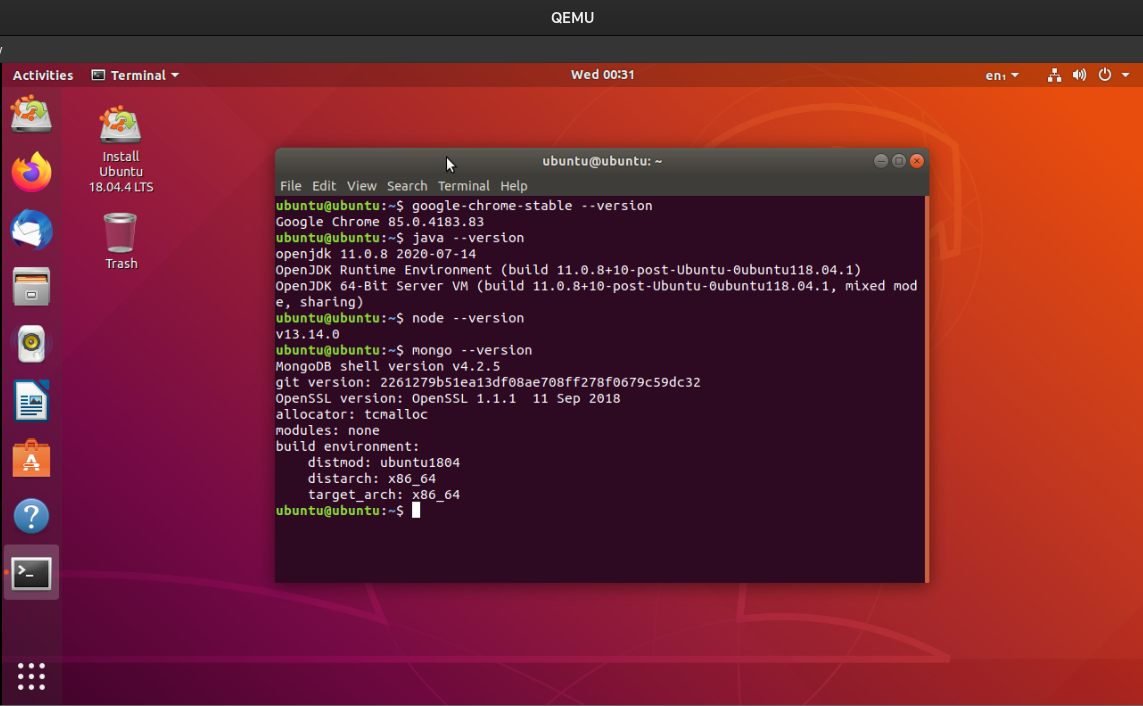
\includegraphics[width=\linewidth]{images/ubuntu-cjmn.png}\\

\chapter*{Zaključak}
\addcontentsline{toc}{chapter}{\numberline{}Zaključak}
\indent
Svakako da bi prostor za poboljšanje bio u kreiranju skripte koja izvršava aktivaciju i deaktivaciju modula, koju bi korisnik mogao pozvati u pokrenutoj live distribuciji. Ova funkcija bi u pozadini trebala da mount-a .squashfs datotečni sistem u zavisnosti od modula koji se aktivira ili deaktivira. Pored toga morala bi i status datoteka biti ažurirana gdje bi se sadržaj status.diff datoteke nadodao u status datoteku.\\
Ova tema je opširna dovoljno da se može proširiti u više smjerova. Demonstriran je proces kreiranja modifikovanih Linux distribucija. Na tu temu se može ići u nedogled jer je moguće modifikovati Linux distribuciju na beskonačno različitih načina.\\
Može se zaključiti da su Linux operativni sistemi podložni modifikaciji u raznim aspektima, vjerovatno u većoj razmjeri nego ostale familije operativnih sistema. To je zasigurno jedan od glavnih razloga za široku upotrebu Linux operativnih sistema, pored glavne činjenice da je Linux open-source.\\
Da se zaključiti također da se Linux distribucije mogu modifikovati za posebne primjene određenoj skupini korisnika te na taj način postići veliku autonomnost i nezavisnost od licenciranih plaćenih softverskih sistema.\\
Možemo zamisliti npr. da Elektrotehnički fakultet premjesti svoj infrastrukturalni sistem u potpunosti u Linux "svijet" počevši od samog nivoa operativnih sistema gdje bi fakultet imao svoj Linux operativni sistem u kom su sve aplikacije namjenski napravljene samo za upotrebu studentima, profesorima i ostatku fakultetskog osoblja. Također kompletan mrežni i aplikativni softver bi treba biti implementiran od pouzdanih inžinjera namjenski samo za potrebe fakulteta.\\
Nedostatak ovog pristupa bi bilo veliko vrijeme izrade i planiranja izvedbe. Također kompleksnost implementacije ovakve infrastrukture je na prvi pogled nepredvidiva. Stoga se ovaj primjer može shvatiti kao imaginaran. Ali on dobro prikazuje upotrebu posebno modifikovanih operativnih sistema.\\
\indent
Tako bi se Linux distribucija mogla modularizirati putem .squashfs datotečnog sistema. Pa možemo zamisliti mogućnost da korisnik prilikom instalacije odabere vrstu korisničkog naloga, npr. student, profesor, ili osoblje, te nakon odabira bi se poseban modul učitao za svaku od ovih različitih uloga. Svakako da bi se dali kreirati različiti moduli za odsjeke i godine studija različitih studentskih grupa. Te bi se ovi moduli mogli učitavati u operativni sistem po potrebi ili po nekom željenom algoritmu.

\chapter*{Reference}
\addcontentsline{toc}{chapter}{\numberline{}Reference}
\indent
Lista članaka i resursa na koje se referencira rad:\\
\url{https://help.ubuntu.com/community/LiveCDCustomization}\\
\url{https://help.ubuntu.com/community/InstallCDCustomization}\\
\url{https://itsfoss.com/customize-xfce/}\\
\url{https://linuxconfig.org/install-gui-on-ubuntu-server-18-04-bionic-beaver}\\
\url{https://www.linuxtrainingacademy.com/install-desktop-on-ubuntu-server/}\\
\url{https://askubuntu.com/questions/378558/unable-to-locate-package-while-trying-to-install-packages-with-apt}\\
\url{http://tldp.org/HOWTO/SquashFS-HOWTO/whatis.html}\\
\url{https://unix.stackexchange.com/questions/166770/unable-to-delete-file-ldlinux-sys-from-a-partition}\\
\url{https://www.digitalocean.com/community/tutorials/how-to-install-node-js-on-ubuntu-18-04}\\
\url{https://itnext.io/how-to-create-a-custom-ubuntu-live-from-scratch-dd3b3f213f81}\\
\url{https://nathanpfry.com/how-to-customize-an-ubuntu-installation-disc/}\\
\url{https://docs.microsoft.com/en-us/azure/app-service/app-service-web-get-started-nodejs}\\
\url{https://phoenixnap.com/kb/how-to-install-lamp-stack-on-ubuntu}\\
\url{https://phoenixnap.com/kb/how-to-install-docker-on-ubuntu-18-04}\\
\url{https://www.digitalocean.com/community/tutorials/how-to-install-mysql-on-ubuntu-18-04}\\
\url{https://linuxize.com/post/how-to-install-mysql-on-ubuntu-18-04/}\\
\url{https://en.wikipedia.org/wiki/Hosts_(file)}\\
\url{https://en.wikipedia.org/wiki/Resolv.conf}\\
\url{https://vitux.com/how-to-install-and-configure-mysql-in-ubuntu-18-04-lts/}\\
\url{https://www.linuxbabe.com/ubuntu/install-google-chrome-ubuntu-18-04-lts}\\
\url{https://stackoverflow.com/questions/11657829/error-2002-hy000-cant-connect-to-local-mysql-server-through-socket-var-run}\\
\url{https://itsfoss.com/install-mysql-ubuntu/}\\
\url{https://www.digitalocean.com/community/tutorials/how-to-install-the-latest-mysql-on-ubuntu-18-04}\\
\url{https://www.digitalocean.com/community/tutorials/how-to-install-mongodb-on-ubuntu-18-04}\\
\url{https://docs.mongodb.com/manual/tutorial/install-mongodb-on-ubuntu/}\\
\url{https://linuxize.com/post/how-to-install-couchdb-on-ubuntu-18-04/}\\
\url{https://www.digitalocean.com/community/tutorials/how-to-install-java-with-apt-on-ubuntu-18-04}\\
\url{https://linuxize.com/post/install-java-on-ubuntu-18-04/}\\
\url{https://www.itzgeek.com/how-tos/linux/ubuntu-how-tos/how-to-install-eclipse-ide-on-ubuntu-18-04-lts.html}\\
\url{https://en.wikipedia.org/wiki/Live_CD}\\
\url{https://en.wikipedia.org/wiki/Comparison_of_file_systems}\\
How To Install Linux to an External USB SSD or HDD - \url{https://www.youtube.com/watch?reload=9&v=glFCEauwGgw}\\
\url{https://askubuntu.com/questions/372607/how-to-create-a-bootable-ubuntu-usb-flash-drive-from-terminal}\\
\url{https://www.howtogeek.com/196051/htg-explains-what-is-a-file-system-and-why-are-there-so-many-of-them/}\\
\url{https://en.wikipedia.org/wiki/File_system}\\
\url{https://www.tldp.org/LDP/sag/html/filesystems.html}\\
\url{https://unix.stackexchange.com/questions/4402/what-is-a-superblock-inode-dentry-and-a-file}\\
\url{https://opensource.com/article/17/5/introduction-ext4-filesystem}\\
\url{https://opensource.com/life/16/10/introduction-linux-filesystems}\\
\url{https://www.slax.org/customize.php}\\
\url{https://www.slax.org/}\\
\url{https://en.wikipedia.org/wiki/Slax}\\
\url{https://en.wikipedia.org/wiki/NimbleX}\\
\url{https://en.wikipedia.org/wiki/Node.js}\\
\url{https://en.wikipedia.org/wiki/Ubuntu}\\

\end{document}
